\chapter{Enclosure}
\label{chapter:enclosure}

\section{Description}

\begin{figure*}
\begin{center}
\ifcoatli
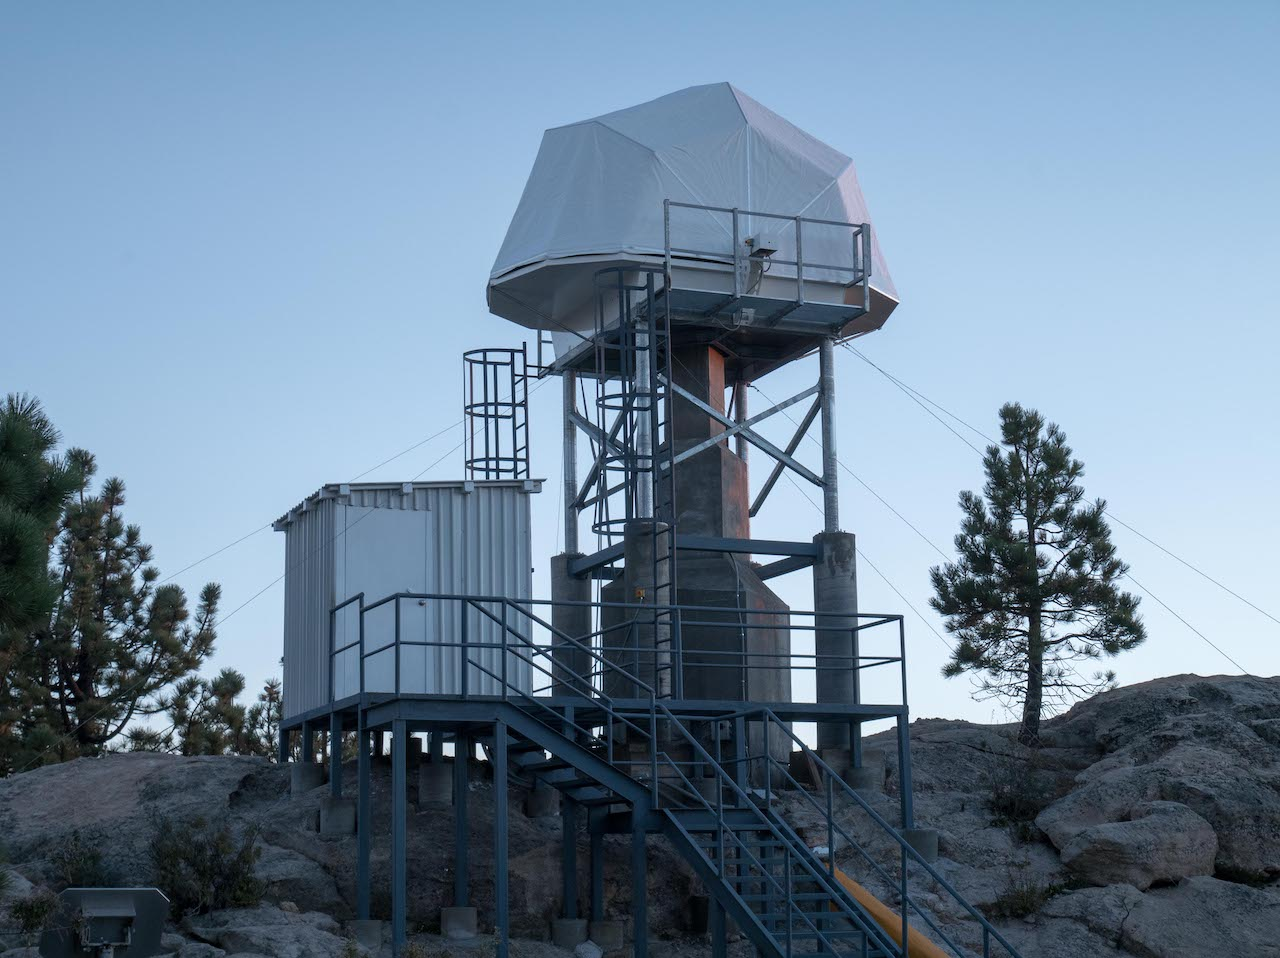
\includegraphics[width=0.8\linewidth]{figures/enclosure-coatli.jpg}
\fi
\ifddoti
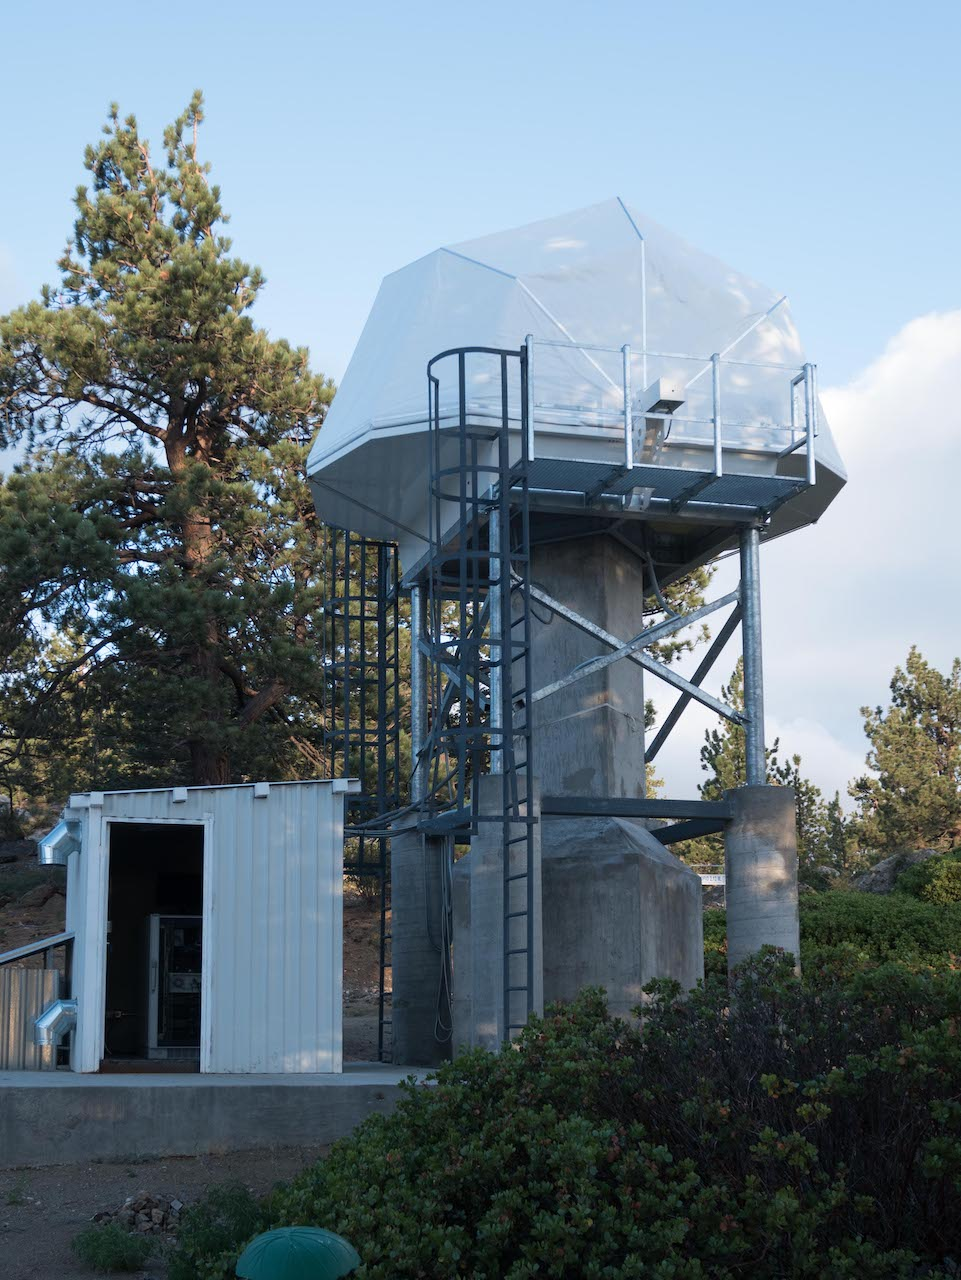
\includegraphics[width=0.8\linewidth]{figures/enclosure-ddoti.jpg}
\fi
\end{center}
\caption{The {\projectname} enclosure.}
\label{figure:enclosure}
\end{figure*}

{\projectname} is protected by an ASTELCO ARTS enclosure, shown in Figure~\ref{figure:enclosure}. The ARTS enclosure consists of a tower, a platform with balconies, and set of folding arches that support a flexible waterproof fabric roof. 

\safety{Under no circumstances ascend to the platform or balconies if the enclosure is in remote mode as the enclosure can close without warning.}

\ifcoatli
The enclosure can open to 60, 120, and 180 $\deg$ and can be controlled locally or remotely. The enclosure is oriented ENE to WSW and opens from the ENE towards the WSW.
\fi
\ifddoti
The enclosure can open to 60, 90, 120, and 180 $\deg$ and can be controlled locally or remotely. The enclosure is oriented NNE to SSW and opens from the NNE towards the SSW.
\fi


The enclosure can open and close in wind speeds of up to 90 km/h and has a survival windspeed of 180 km/h.

\begin{figure*}
\begin{center}
\ifcoatli
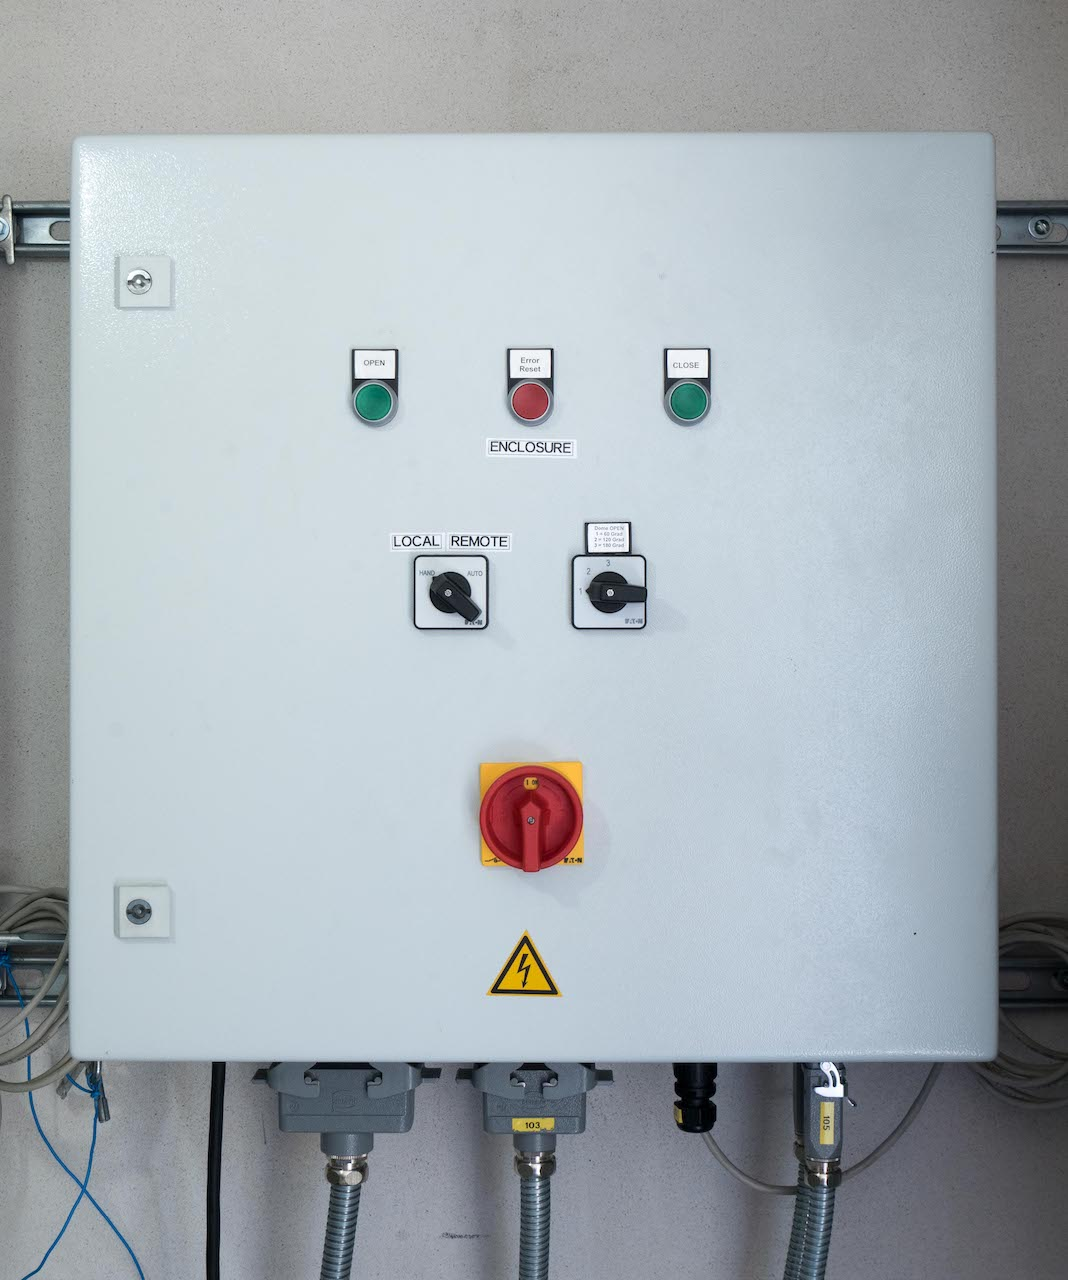
\includegraphics[width=0.6\linewidth]{figures/enclosure-coatli-controller.jpg}
\fi
\ifddoti
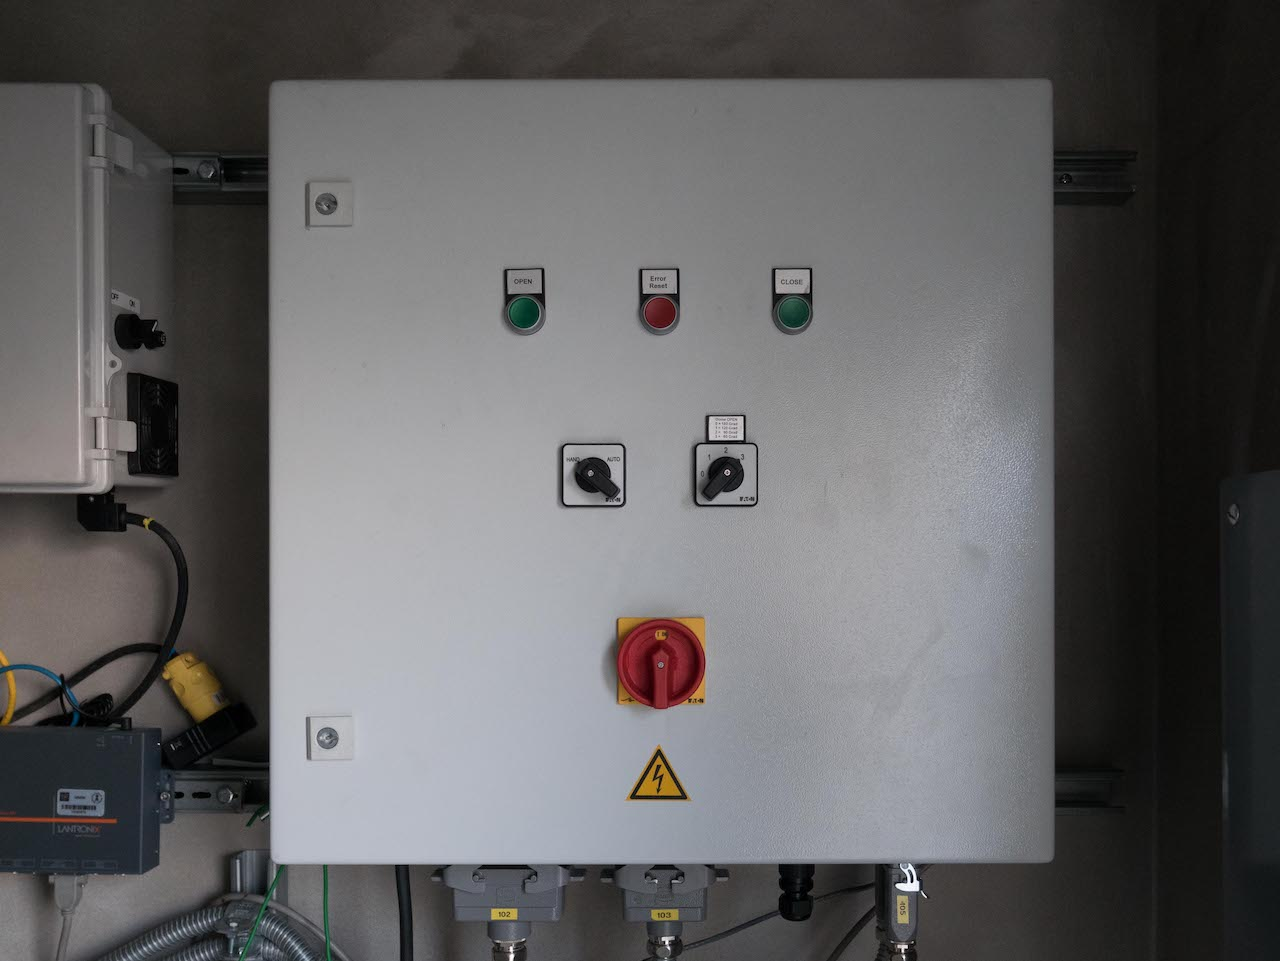
\includegraphics[width=0.6\linewidth]{figures/enclosure-ddoti-controller.jpg}
\fi
\end{center}
\caption{The enclosure controller in the shed.}
\label{figure:enclosure-controller}
\end{figure*}

The controller for the enclosure, shown in Figure~\ref{figure:enclosure-controller} is located in a cabinet in the shed. The enclosure is opened and closed by two geared motors, one on each balcony. The position is sensed by proximity sensors on the bearings (fully open and partially open positions) and at the point that the last arch closes (closed position). The controller and the motors are powered by 220 V 60 Hz from the Circuit A via the 220 V UPS and 220 V iBootBar.

\begin{figure*}
\begin{center}
\resizebox{\columnwidth}{!}{%
\begin{labeled}{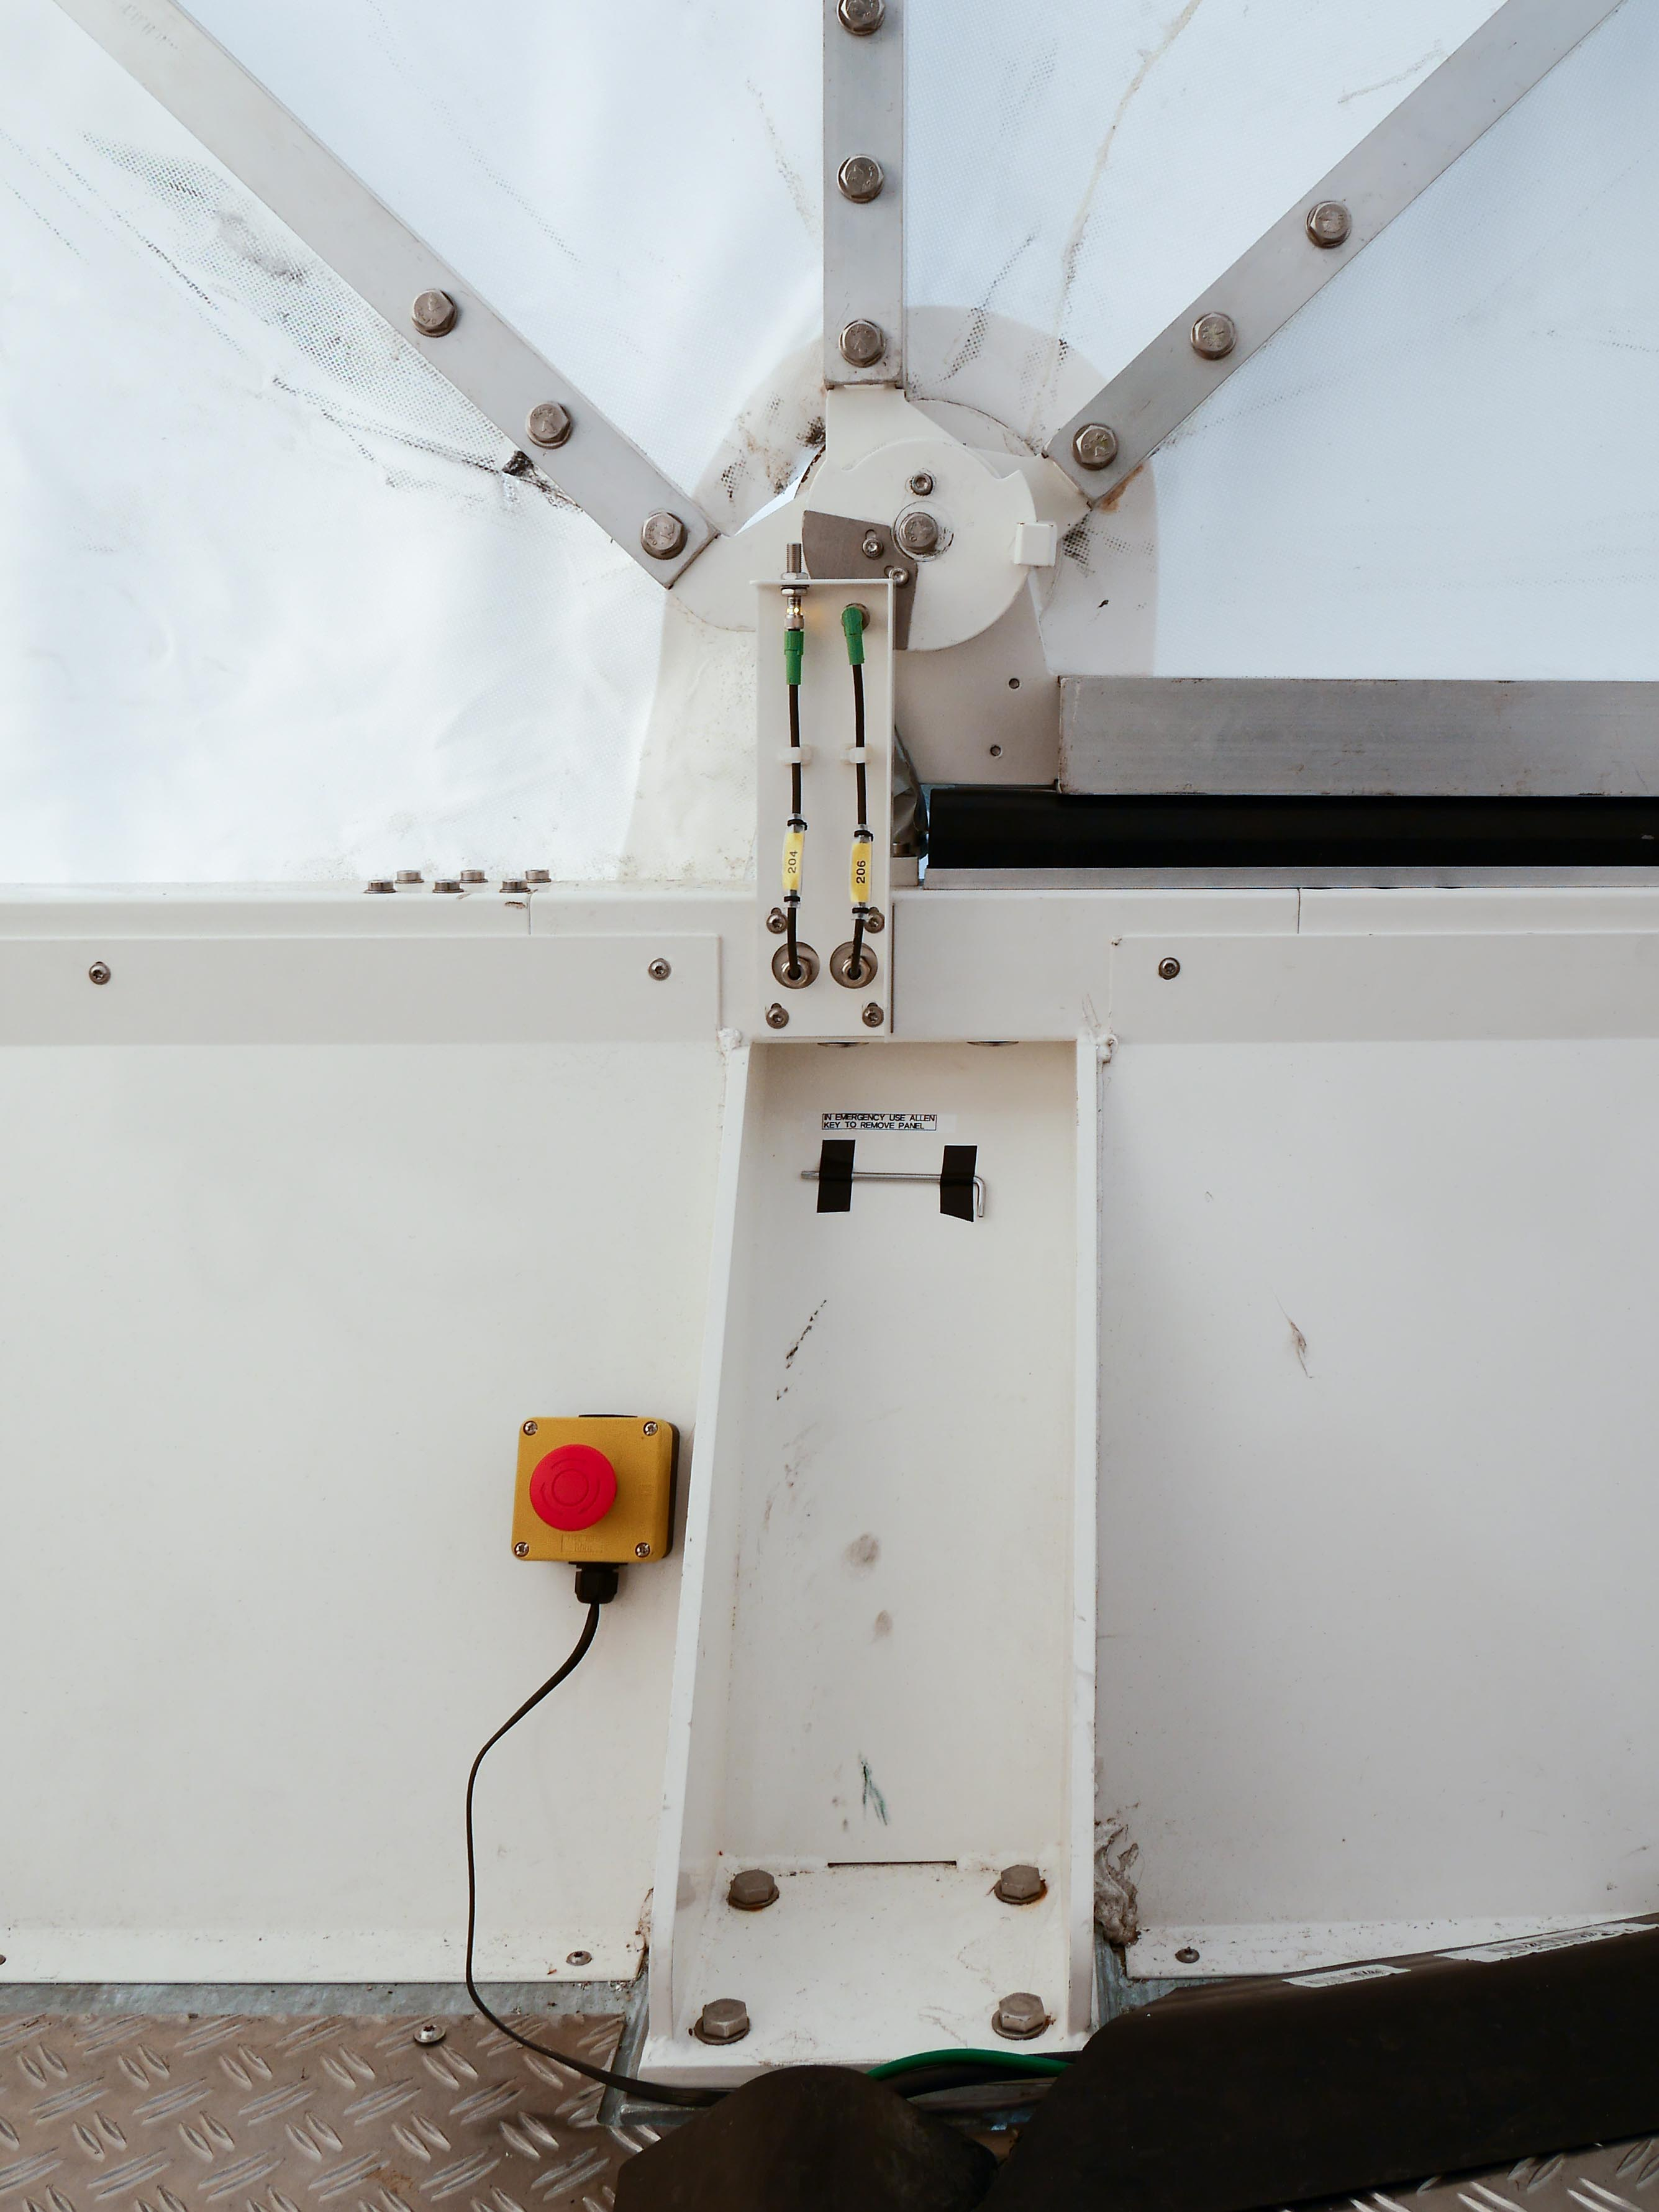
\includegraphics[width=0.48\linewidth]{figures/enclosure-bearing-north.jpg}}
\arrowandlabel{(-0.9,-1.7)}{(-1.2,-4)}{north}{Emergency Button};
\arrowandlabel{(+0.3,-0.4)}{(+1.8,-4)}{north}{Allen Key};
\arrowandlabel{(+0.0,+2.1)}{(0,+4)}{south}{Proximity Sensors};
\end{labeled}
\space
\begin{labeled}{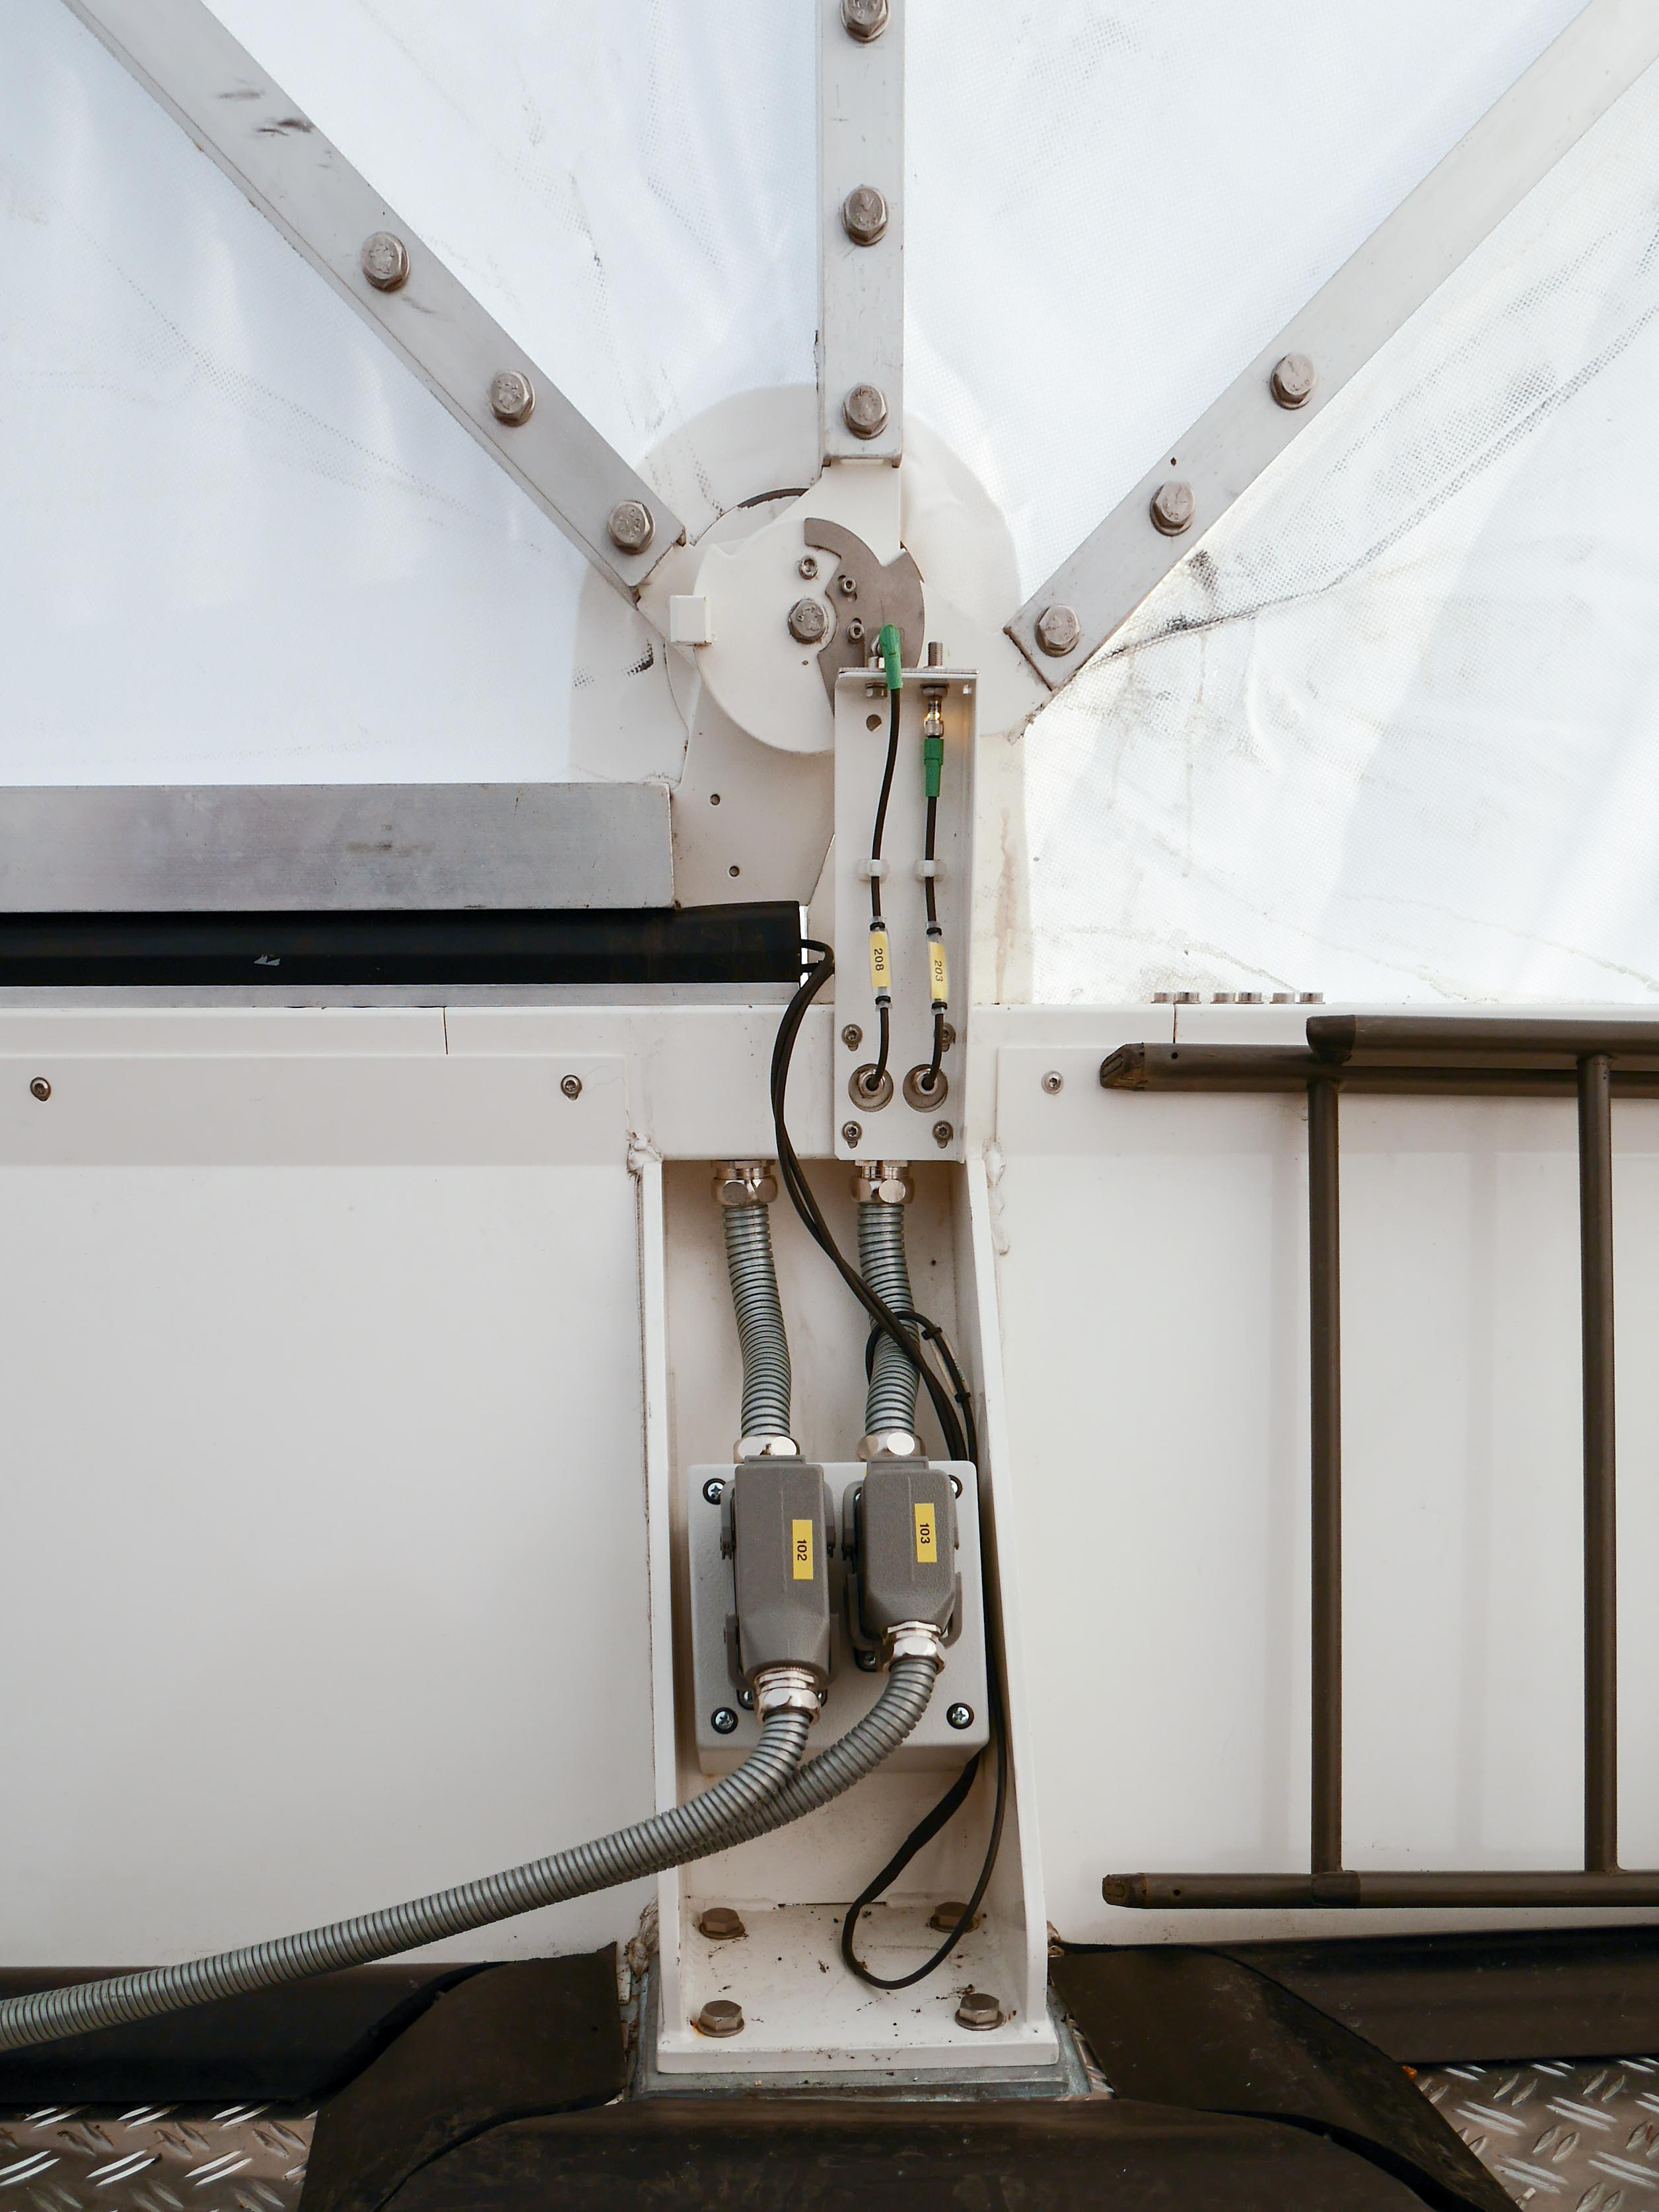
\includegraphics[width=0.48\linewidth]{figures/enclosure-bearing-south.jpg}}
\arrowandlabel{(0.2,+2.1)}{(0.2,+4)}{south}{Proximity Sensors};
\dummylabel{(-1.2,-4)}{north}
\end{labeled}}
\end{center}
\caption{The north (left) and south (right) bearings for the folding roof. Notice the proximity sensors, the emergency stop button for the mount, and the Allen key to escape in an emergency.
\ifddoti
The COATLI installation is shown, but the DDOTI installation is similar.
\fi
}
\label{figure:enclosure-bearing-north}
\label{figure:enclosure-beating-south}
\end{figure*}


\begin{figure*}
\begin{center}
\begin{labeled}{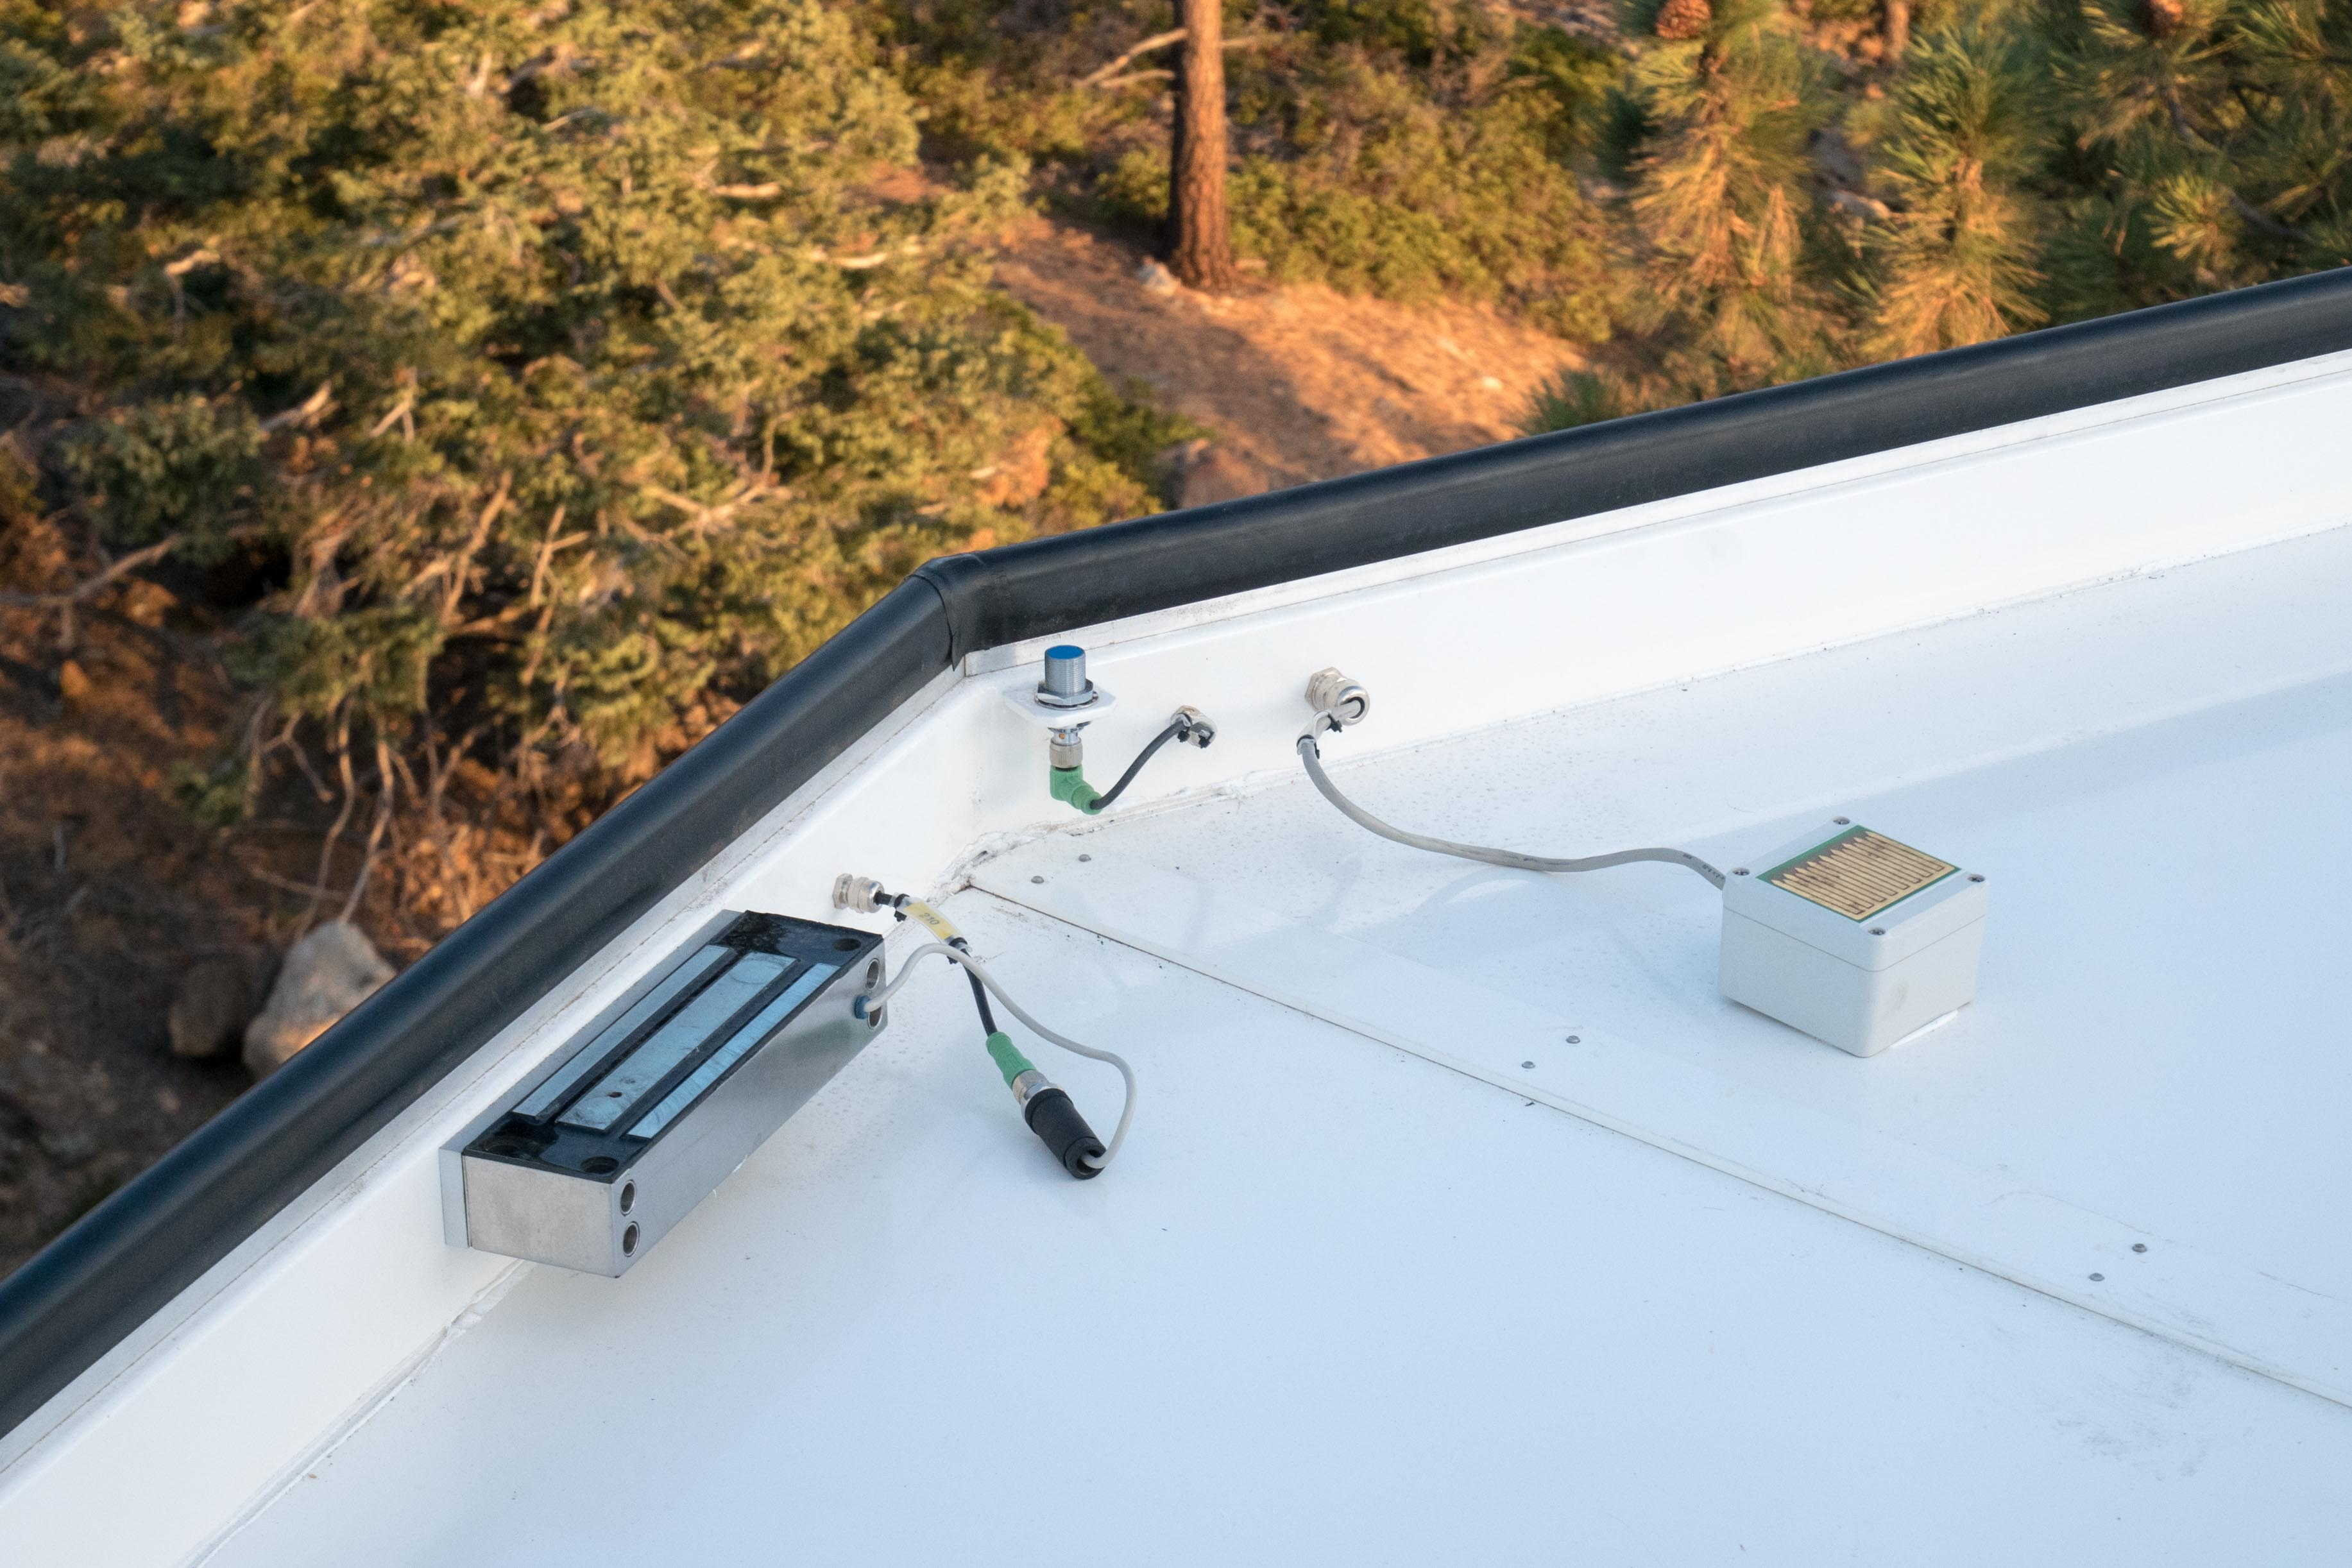
\includegraphics[width=0.8\linewidth]{figures/enclosure-electromagnetic-lock.jpg}}
\arrowandlabel{(-0.45,+0.7)}{(-0.45,+4)}{south}{Proximity Sensor}
\arrowandlabel{(-2.0,-2.0)}{(-2,-4)}{north}{Electromagnetic Lock};
\arrowandlabel{(+2.7,-1.2)}{(+2.7,-4)}{north}{Rain Sensor};
\end{labeled}
\end{center}
\caption{The enclosure electromagnetic lock (left), 0 $\deg$ proximity sensor (the cylinder with the blue top in the center), and rain sensor (the white box with the copper contacts on the right).
\ifddoti
The COATLI installation is shown, but the DDOTI installation is similar.
\fi
}
\label{figure:enclosure-electromagnetic-lock}
\end{figure*}

The enclosure has an electromagnetic lock, shown in Figure~\ref{figure:enclosure-electromagnetic-lock}, that holds it firmly closed. If the lock is not activated, the wind can open the roof a few centimeters and allow the ingress of rain or snow.

\safety{The enclosure controller should normally be switched on at all times in order to keep the electromagnetic lock activated.}

The electromagnet that holds the enclosure closed is normally activated by the PLC. However, we have modified the controller to add a switch inside the controller that switches on the enclosure electromagnet and actuates the enclosure emergency stop buttons. This ensures that the electromagnet stays energized even if the PLC fails and that the PLC cannot attempt to open the enclosure. This switch is shown in Figure~\ref{figure:enclosure-controller-manual-lock-switch}.

\begin{figure*}
\begin{center}
\ifcoatli
\resizebox{\columnwidth}{!}{%
\begin{labeled}{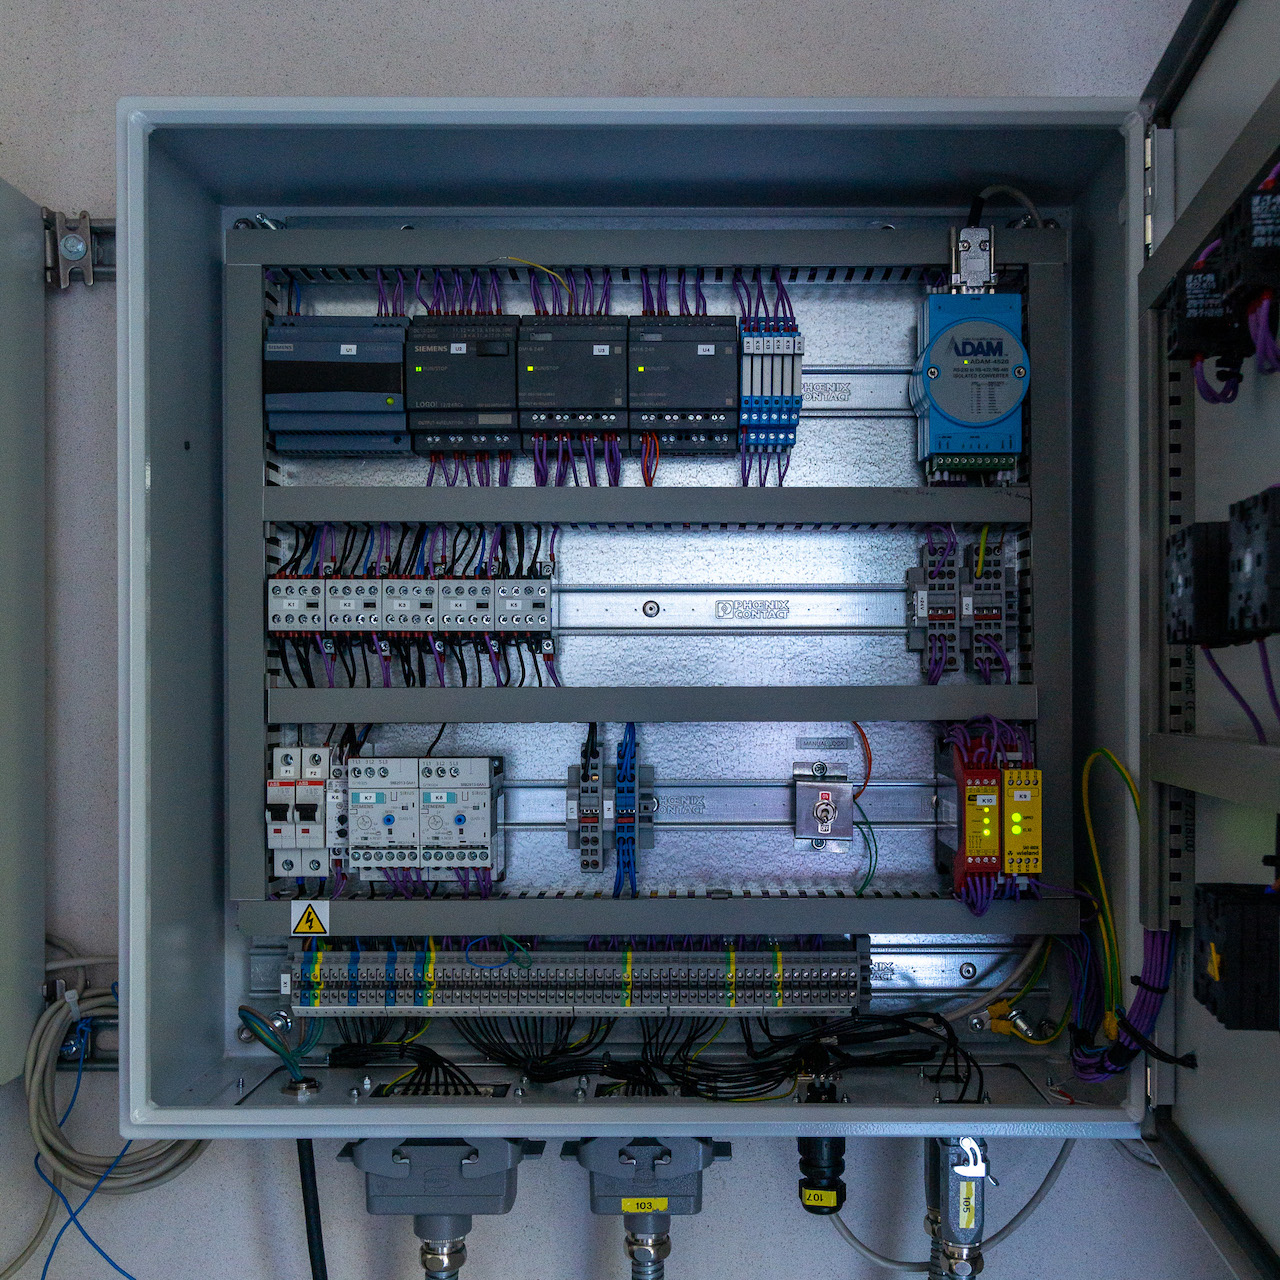
\includegraphics[width=\linewidth]{figures/enclosure-controller-inside-coatli.jpg}}
\arrowandlabel{(+1.75,-2.0)}{(+1.75,-6.5)}{north}{Manual Lock Switch};
\end{labeled}}
\fi
\ifddoti
\resizebox{\columnwidth}{!}{%
\begin{labeled}{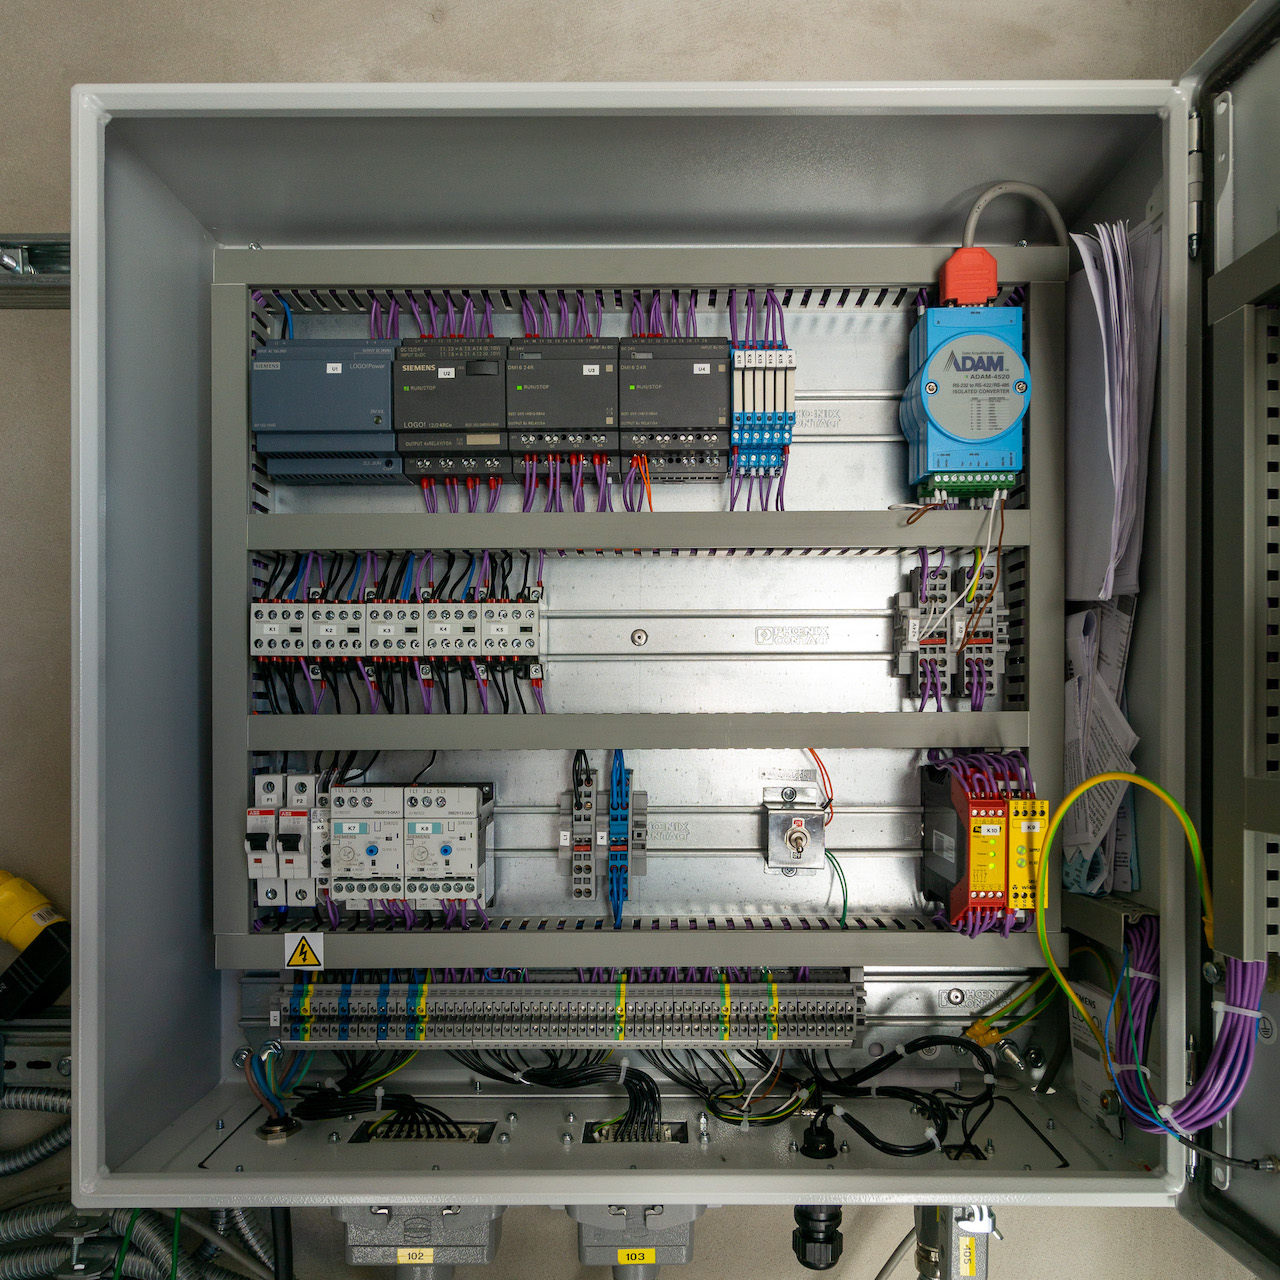
\includegraphics[width=\linewidth]{figures/enclosure-controller-inside-ddoti.jpg}}
\arrowandlabel{(+1.5,-2.3)}{(+1.5,-6.5)}{north}{Manual Lock Switch};
\end{labeled}}
\fi
\end{center}
\caption{The inside of the enclosure controller cabinet showing the manual switch for the electromagnet.}
\label{figure:enclosure-controller-manual-lock-switch}
\end{figure*}

The enclosure has a rain sensor, also shown in Figure~\ref{figure:enclosure-electromagnetic-lock}. In automatic mode, it will automatically close if the rain sensor gets wet.

\begin{figure*}
\begin{center}
\begin{labeled}{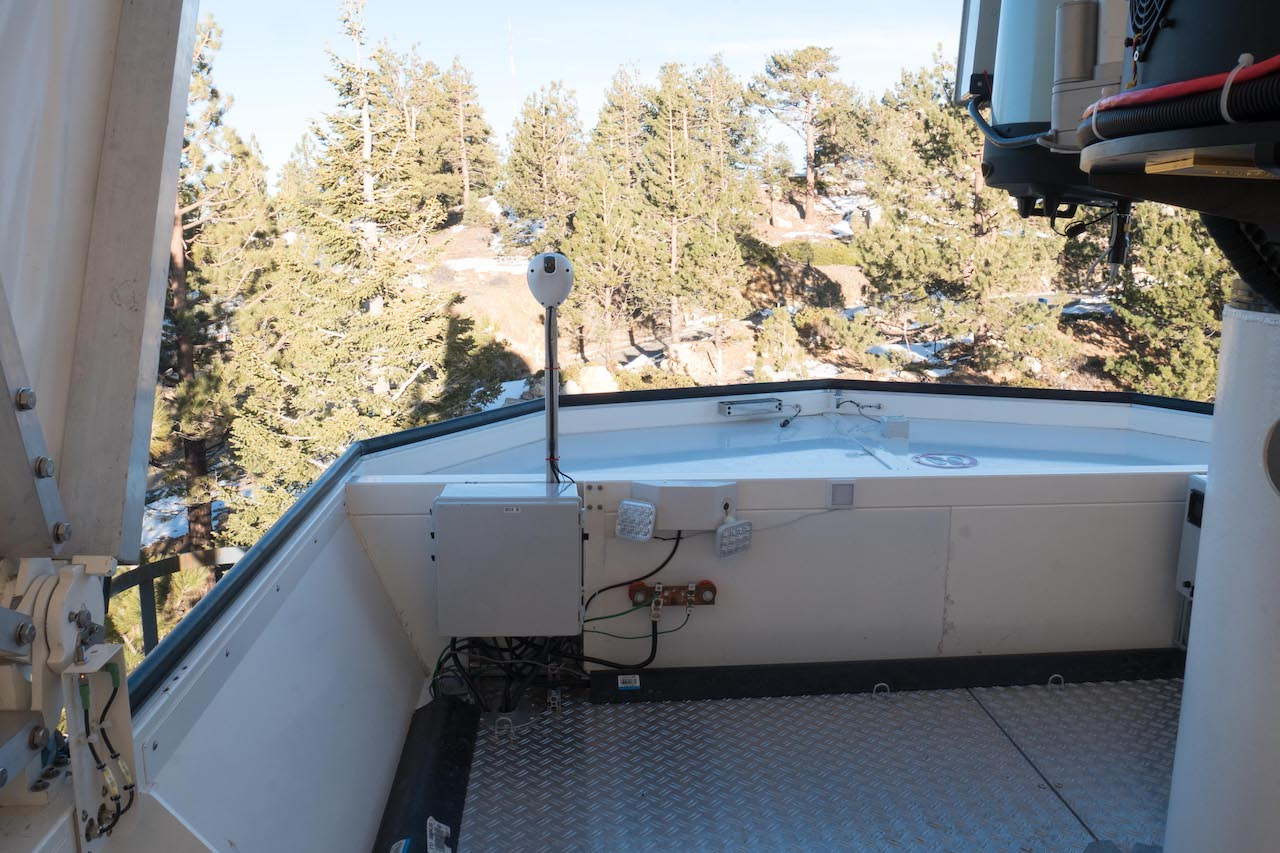
\includegraphics[width=0.8\linewidth]{figures/enclosure-safety-seal.jpg}}
\arrowonly{(-0.2,+0.4)}{(-0.45,+4)}{south};
\arrowonly{(-3.0,-0.9)}{(-0.45,+4)}{south};
\arrowandlabel{(+3.0,+0.4)}{(-0.45,+4)}{south}{Safety Seal};
\end{labeled}
\end{center}
\caption{The enclosure safety seal, the black rubber seal on the lower edge of the enclosure opening. If this is pressed, the motors will stop and an error is set in the controller.
\ifddoti
The COATLI installation is shown, but the DDOTI installation is similar.
\fi
}
\label{figure:enclosure-safety-seal}
\end{figure*}

The enclosure has a safety seal along the lower edge of the opening. The motors will stop if this is pressed. This avoids the enclosure closing on someone or something. However, it is easy to activate the safety rail when entering or leaving the enclosure. 

\begin{figure*}
\begin{center}
\resizebox{\columnwidth}{!}{%
\begin{labeled}{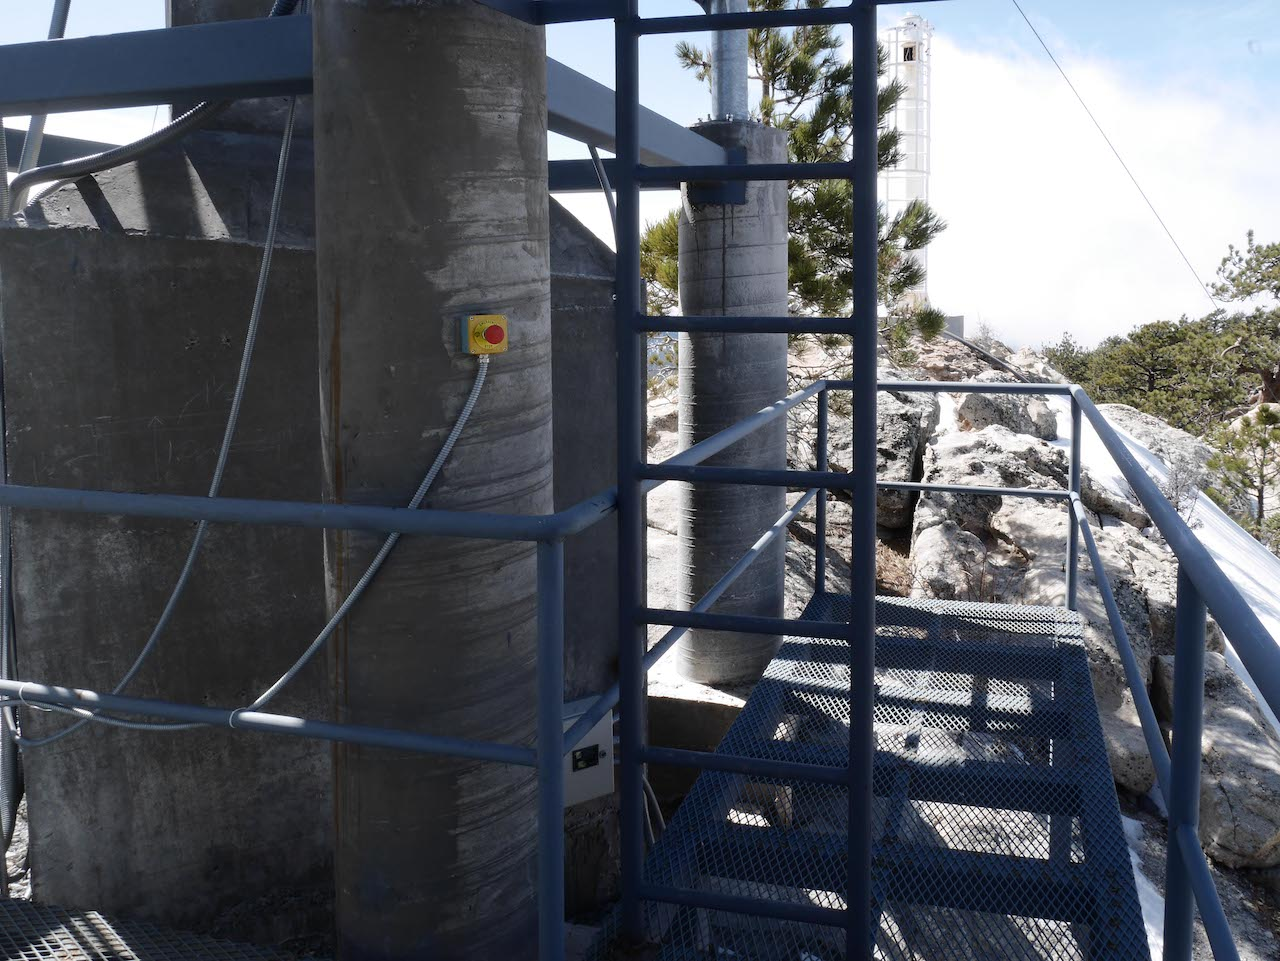
\includegraphics[width=0.48\linewidth]{figures/enclosure-emergency-stop-lower.jpg}}
\arrowandlabel{(-0.7,+0.8)}{(-0.7,+2.5)}{south}{Emergency Button};
\end{labeled}
\space
\begin{labeled}{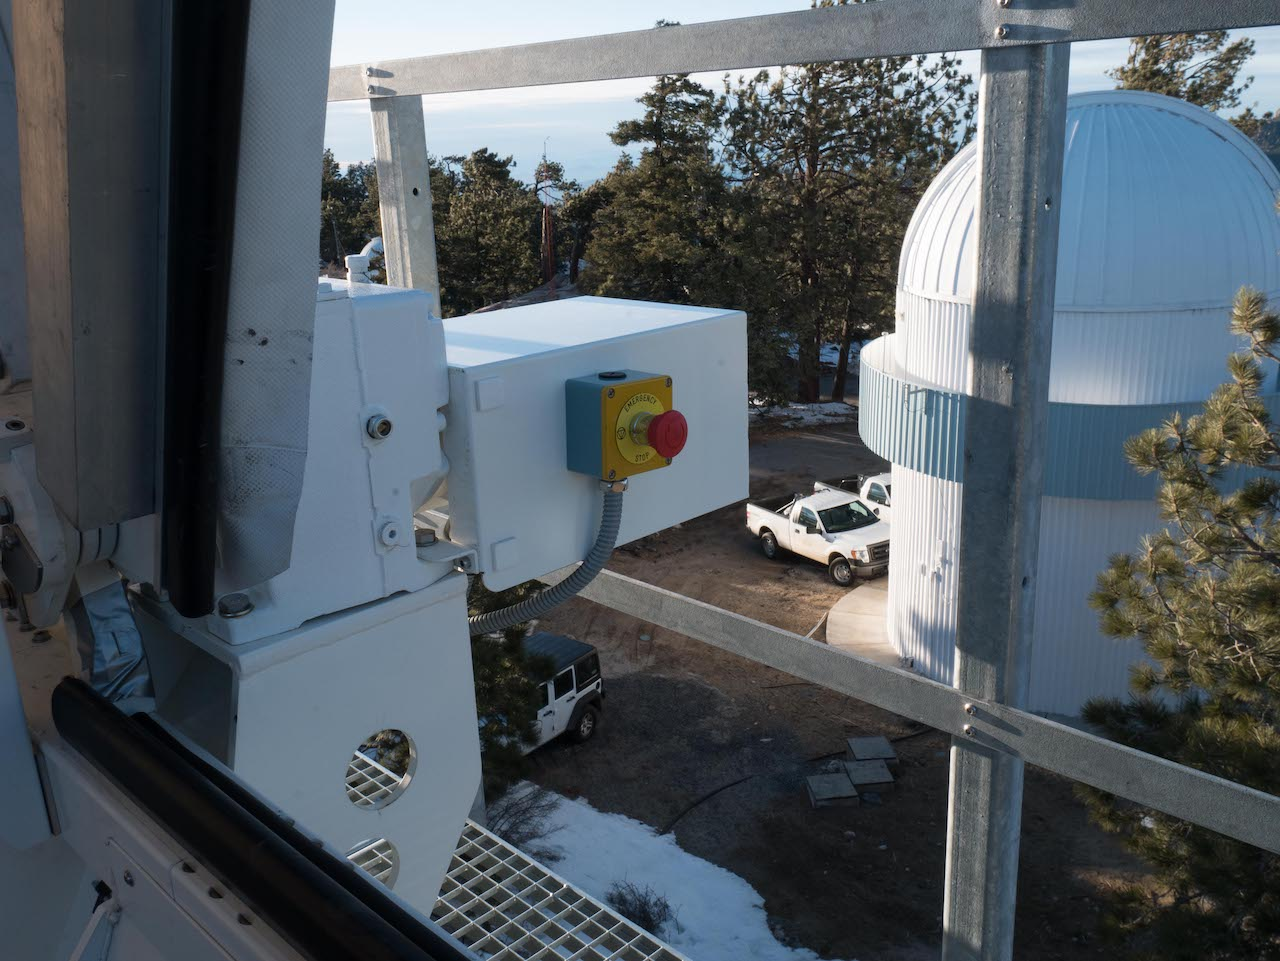
\includegraphics[width=0.48\linewidth]{figures/enclosure-emergency-stop-upper.jpg}}
\arrowandlabel{(-0.0,+0.4)}{(-0.0,+2.5)}{south}{Emergency Button};
\end{labeled}}
\end{center}
\caption{The enclosure emergency stop buttons, next to the main access ladder (left) and on the northern motor cowling (right).
\ifddoti
The COATLI installation is shown, but the DDOTI installation is similar.
\fi
}
\label{figure:enclosure-emergency-stop}
\end{figure*}

The enclosure also has two emergency stop buttons, one at the bottom of the main access ladder and the other on the northern motor cowling. These are shown in Figure~\ref{figure:enclosure-emergency-stop}. Again, the motors will stop if either of these are pressed.

\begin{figure*}
\begin{center}
\resizebox{\columnwidth}{!}{%
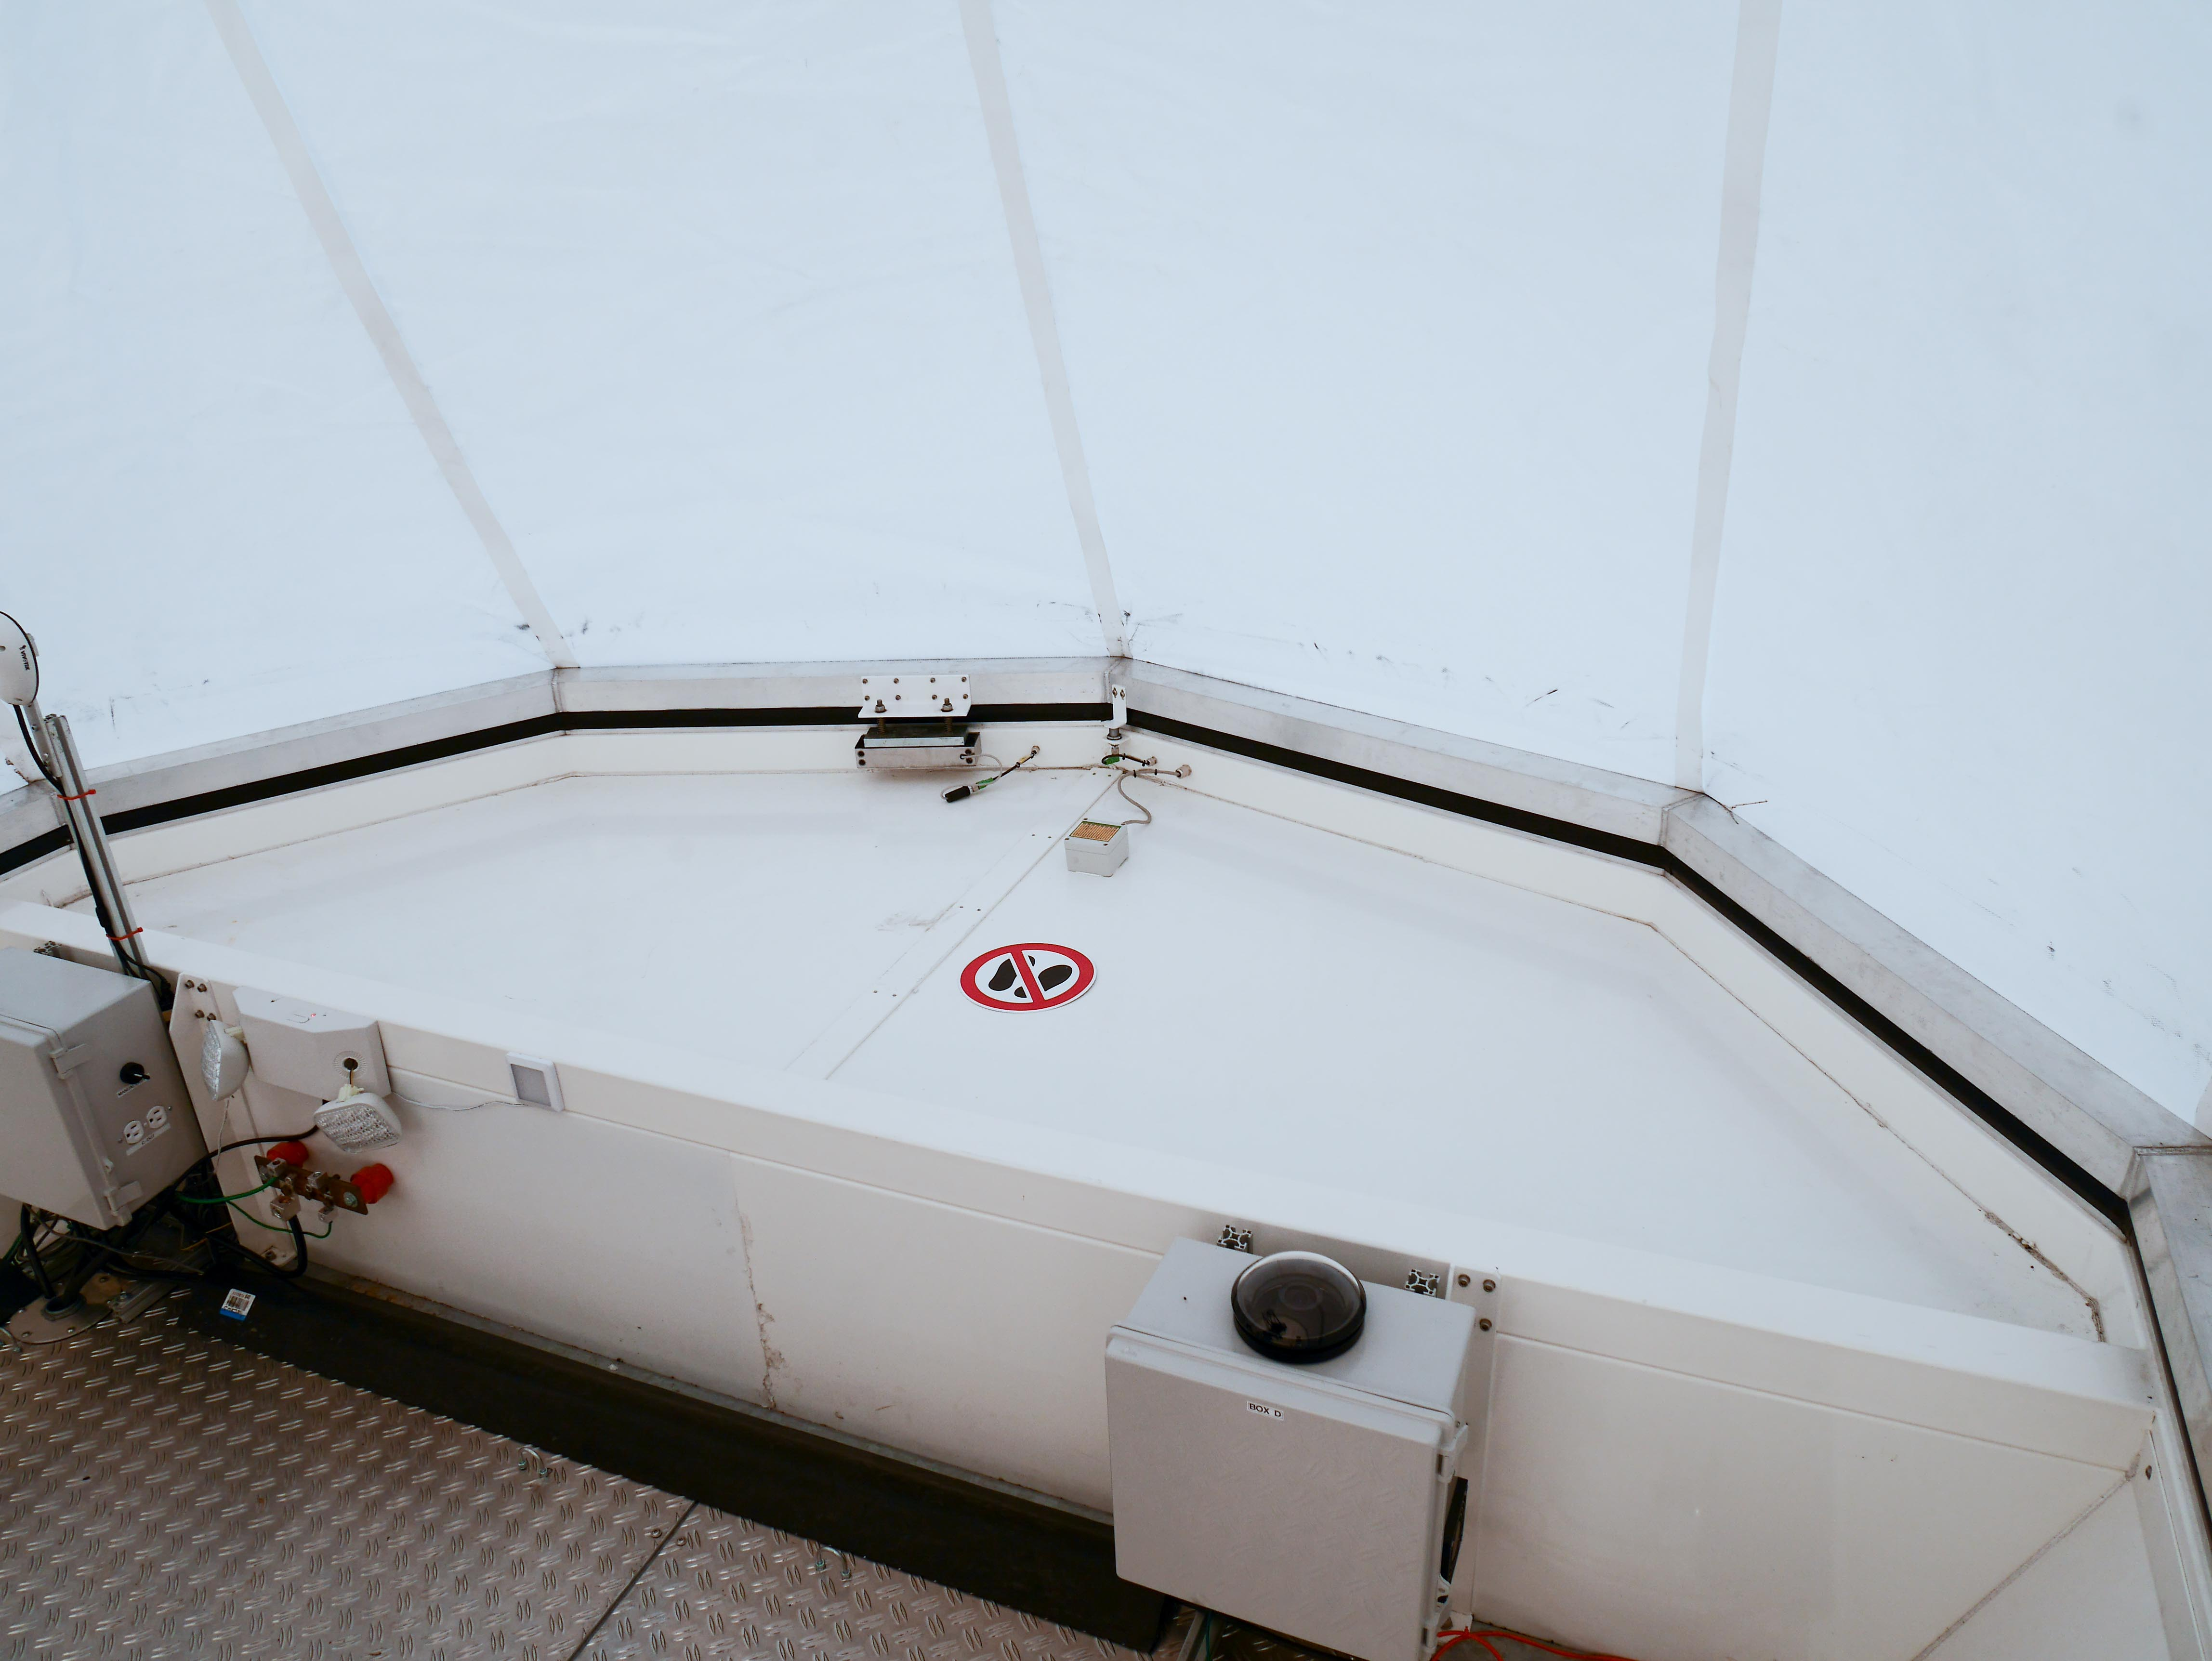
\includegraphics[width=0.48\linewidth]{figures/enclosure-elevated-east.jpg}%
\space
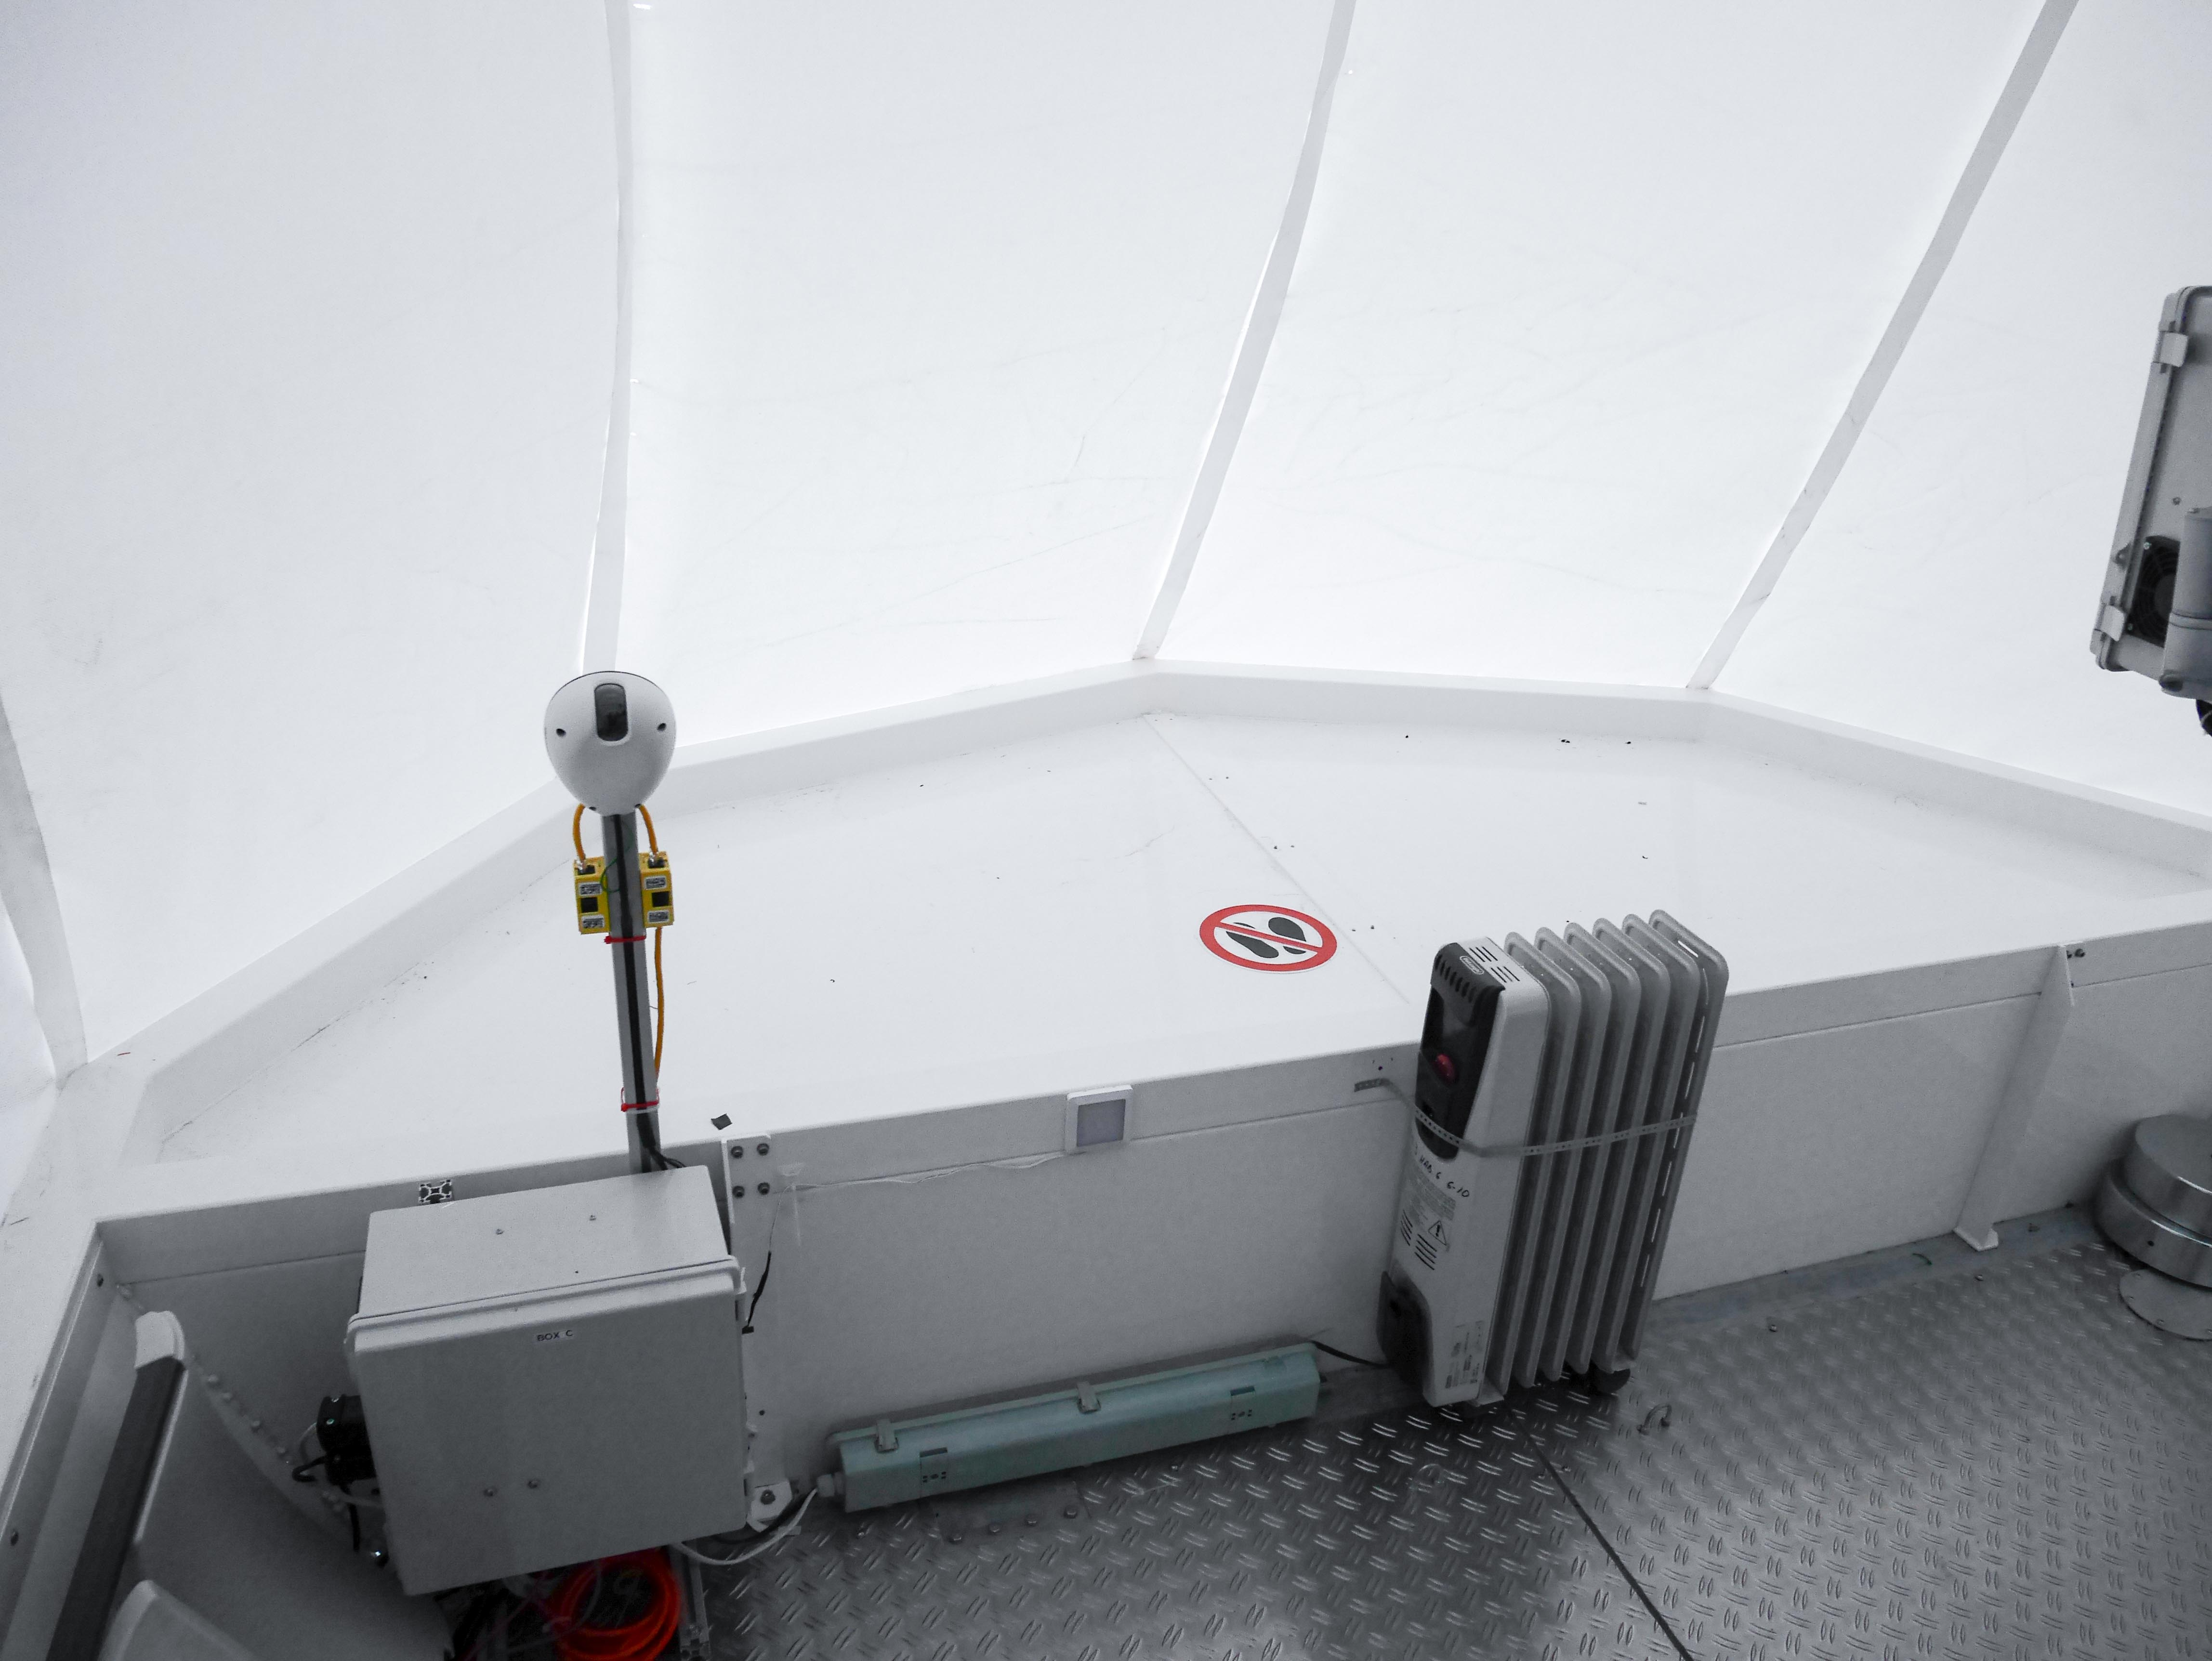
\includegraphics[width=0.48\linewidth]{figures/enclosure-elevated-west.jpg}%
}
\end{center}
\caption{Do not walk on the elevated areas at the ends of the platform as they are not load bearing. Note the “no step” signs.
\ifddoti
The COATLI installation is shown, but the DDOTI installation is similar.
\fi
}
\label{figure:enclosure-elevated}
\end{figure*}

The two semi-circular elevated areas at the ends of the platform, shown in Figure~\ref{figure:enclosure-elevated}, are not load bearing and are marked with “no step” signs. If you attempt to walk on these, you will likely fall.

\safety{Do not walk on the elevated areas at the ends of the platform!}

If you are trapped in the enclosure and cannot summon help, you can escape by using the Allen key taped below the northern bearing to remove one of the sloping side panels to gain access to the balcony. See Figure~\ref{figure:enclosure-bearing-north}.

\begin{figure*}
\begin{center}
\ifcoatli
\resizebox{\linewidth}{!}{\begin{labeled}{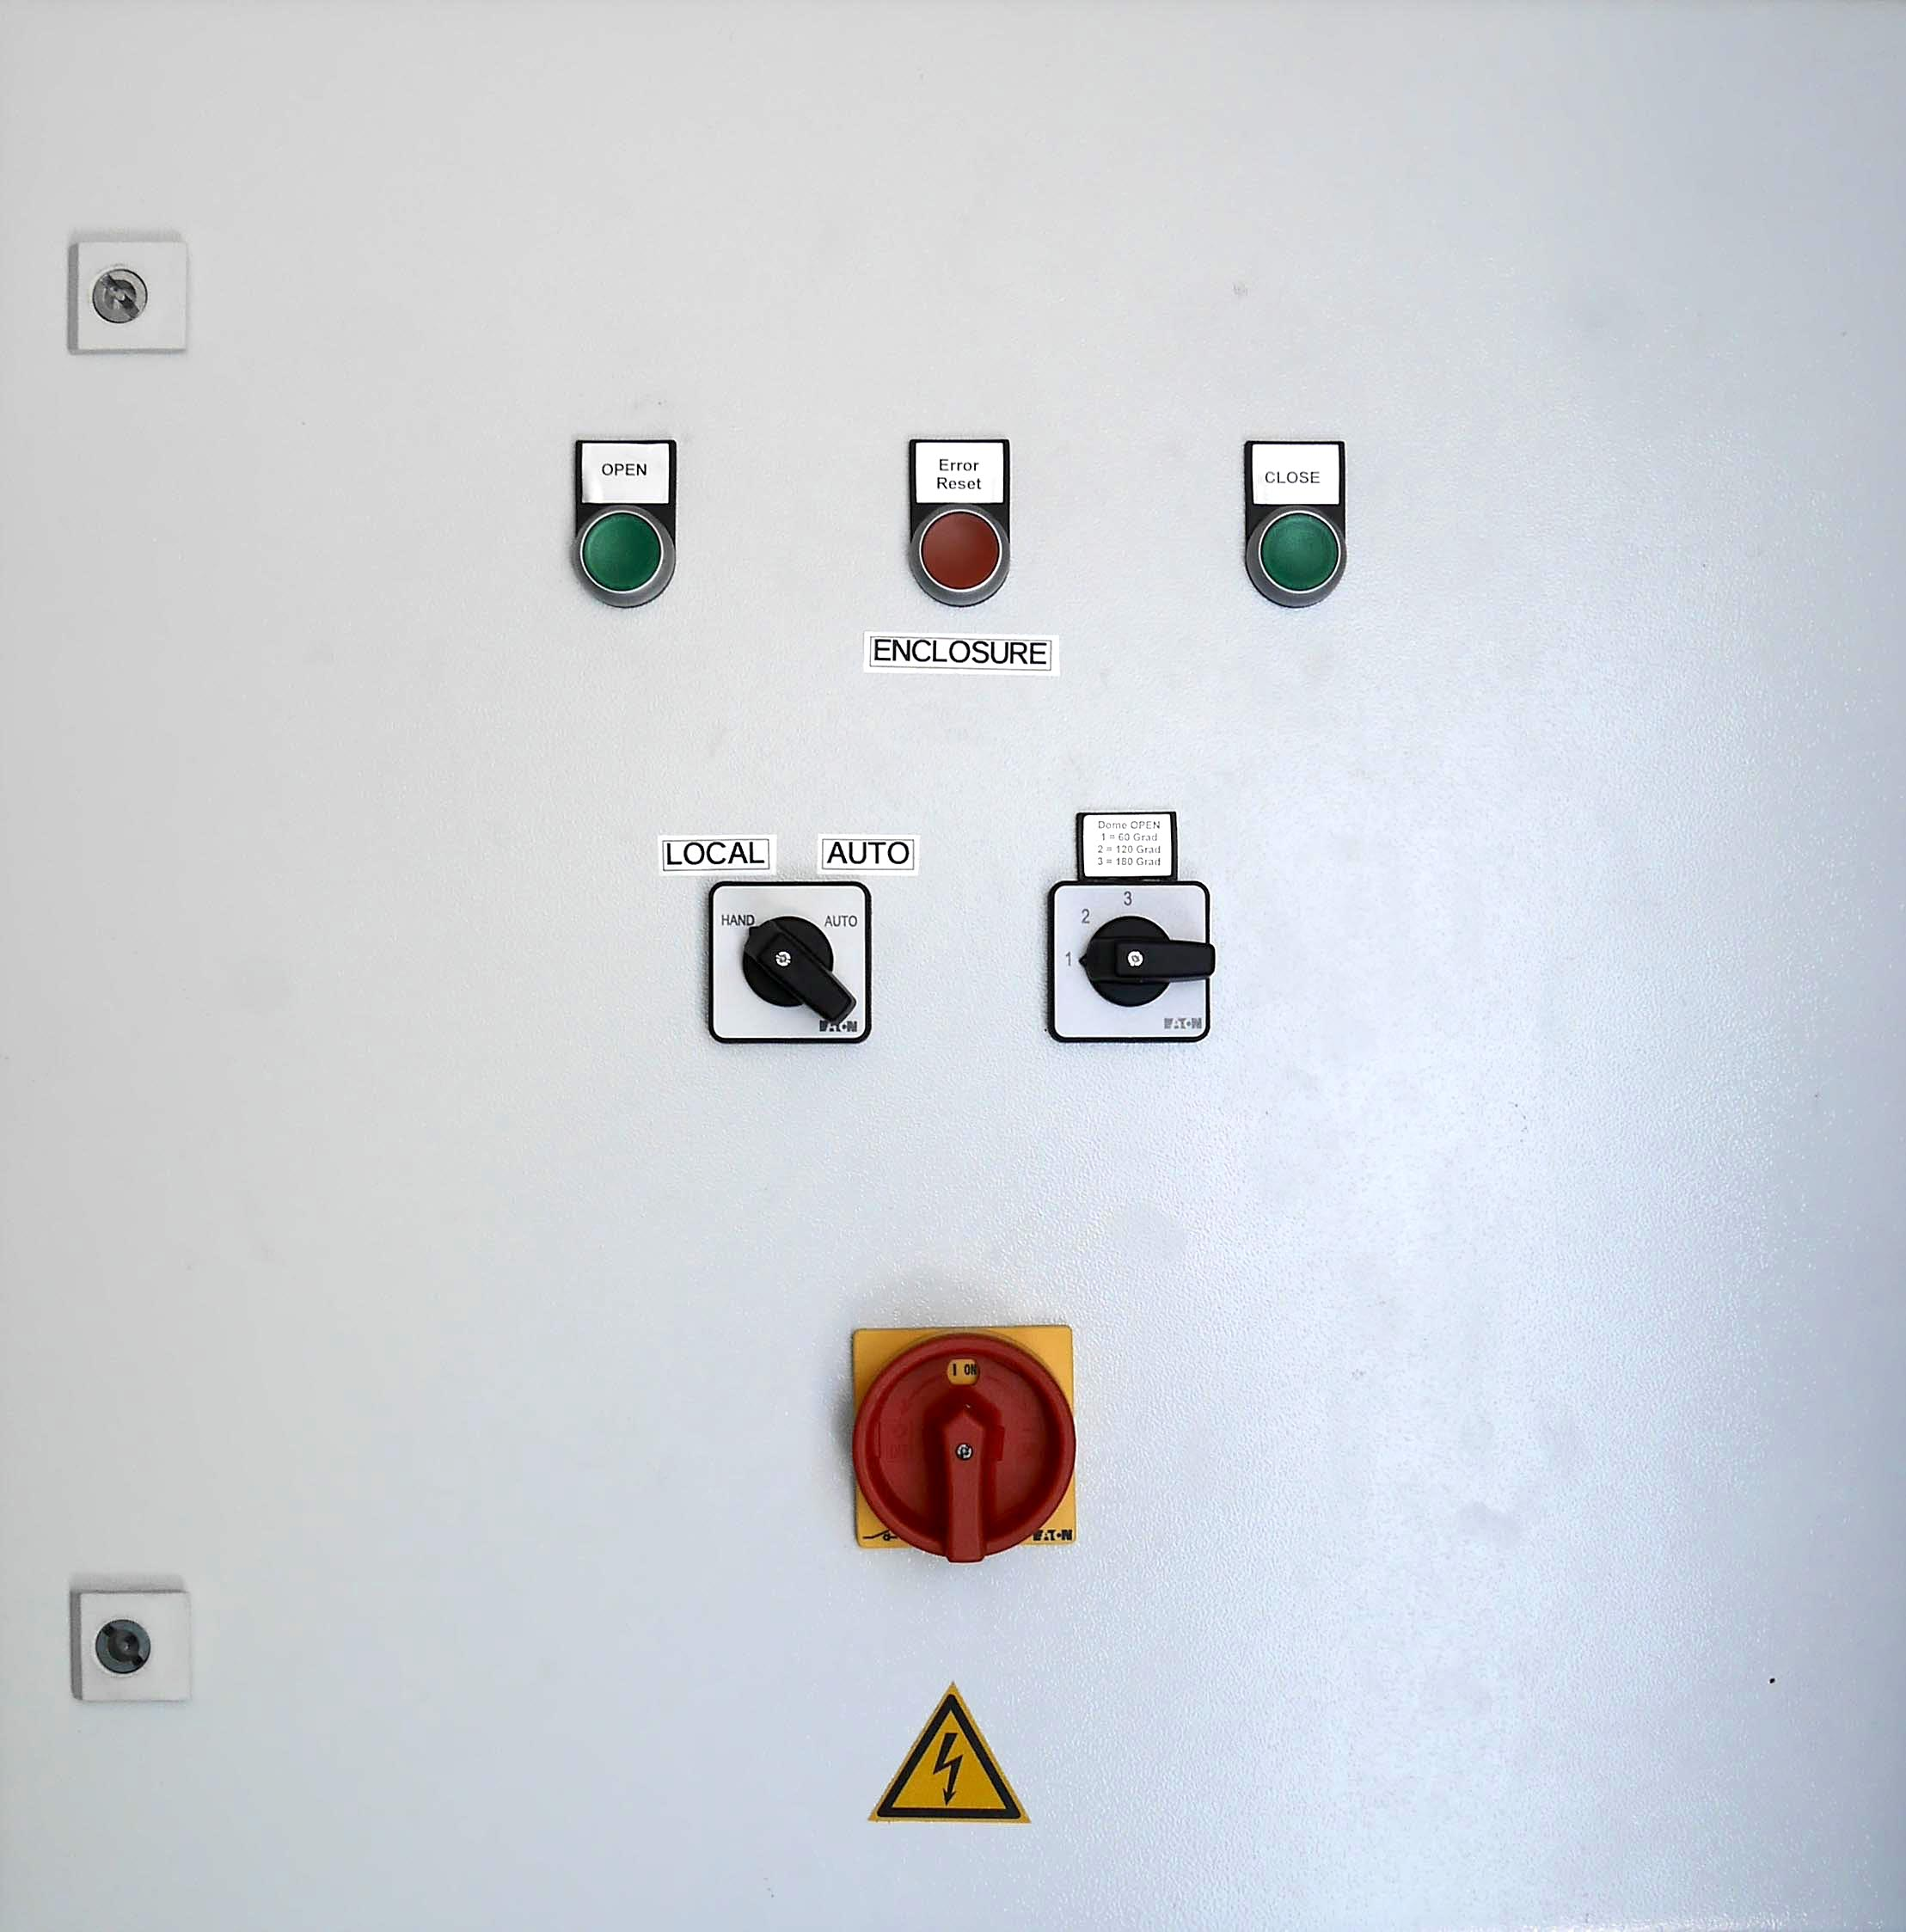
\includegraphics[width=\linewidth]{figures/enclosure-coatli-controller-door.jpg}}
%\draw[dotted] (-5,-5) grid (+5,+5);
\arrowandlabel{(-1.1,-0.6)}{(-4.0,-6.4)}{north}{Mode Selector Switch};
\arrowandlabel{(+1.1,-0.6)}{(+4.0,-6.4)}{north}{Angle Selector Switch};
\arrowandlabel{(+0.0,-4.0)}{(+0.0,-6.4)}{north}{Main Power Switch};
\arrowandlabel{(-2.1,+3.5)}{(-3.0,+6.4)}{south}{Open Button};
\arrowandlabel{(+2.2,+3.5)}{(+3.0,+6.4)}{south}{Close Button};
\arrowandlabel{(+0.0,+3.5)}{(+0.0,+6.4)}{south}{Error Button};
\end{labeled}}
\fi
\ifddoti
\resizebox{\linewidth}{!}{\begin{labeled}{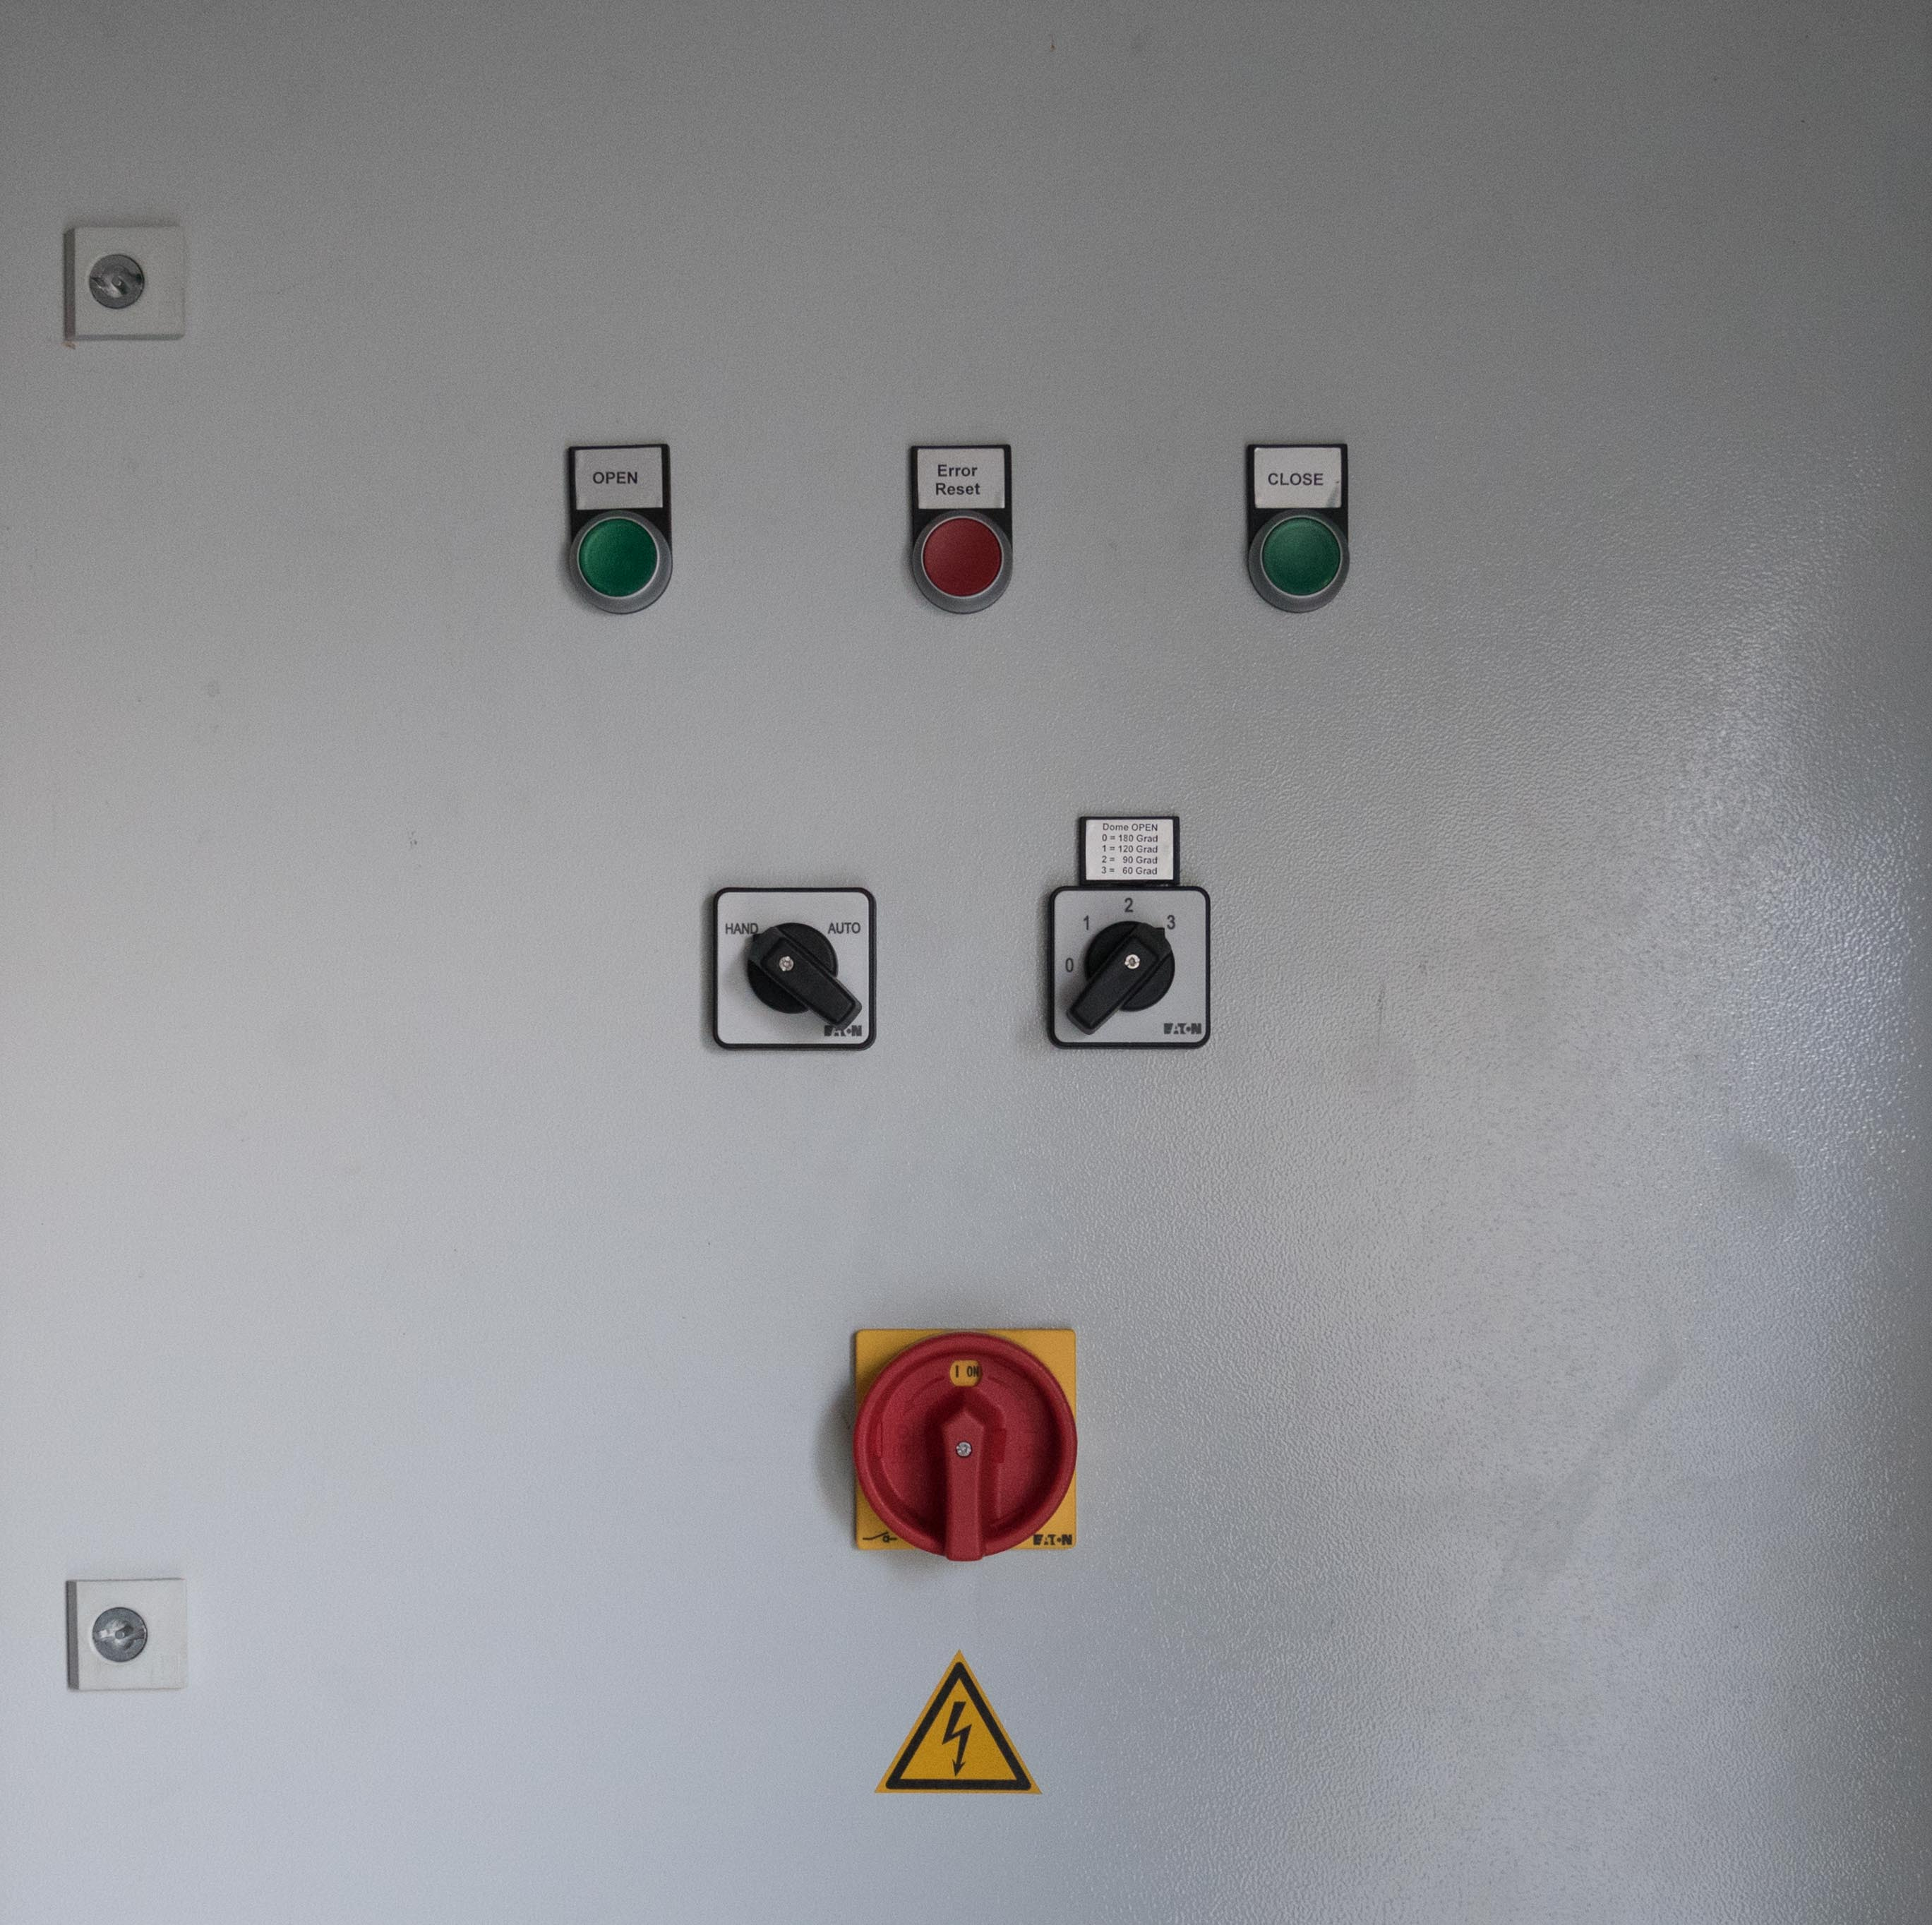
\includegraphics[width=\linewidth]{figures/enclosure-ddoti-controller-door.jpg}}
%\draw[dotted] (-5,-5) grid (+5,+5);
\arrowandlabel{(-1.1,-0.6)}{(-4.0,-6.4)}{north}{Mode Selector Switch};
\arrowandlabel{(+1.1,-0.6)}{(+4.0,-6.4)}{north}{Angle Selector Switch};
\arrowandlabel{(+0.0,-4.0)}{(+0.0,-6.4)}{north}{Main Power Switch};
\arrowandlabel{(-2.1,+3.5)}{(-3.0,+6.4)}{south}{Open Button};
\arrowandlabel{(+2.2,+3.5)}{(+3.0,+6.4)}{south}{Close Button};
\arrowandlabel{(+0.0,+3.5)}{(+0.0,+6.4)}{south}{Error Button};
\end{labeled}}
\fi
\end{center}
\caption{The enclosure controller door and control panel. Bottom: the main power switch. Middle row, left to right: the mode selector switch (“LOCAL” and “REMOTE”) and the angle selector switch (180 $\deg$ is fully open). Top row, left to right: the open button, the error button, and the close button.
}
\label{figure:enclosure-controller-door}
\end{figure*}

The enclosure controller can be in remote or local mode. The mode is selected by the switch on the door of the enclosure controller in the shed (see Figure~\ref{figure:enclosure-controller-door}). In remote mode:
\begin{itemize}
\item
The switches on the enclosure controller to open and close the enclosure and to reset errors are deactivated.
\item
The robotic control system can open and close. 
\item
The enclosure will close automatically if the rain sensor gets wet.
\end{itemize}
In local mode:
\begin{itemize}
\item
The switches on the enclosure controller to open and close the enclosure and to reset errors are active.
\item
The robotic control system cannot open or close. 
\item
The enclosure will not close if the rain sensor gets wet.
\end{itemize}

If there is an error, the red error button on the enclosure controller will flash or be constantly lit. The interpretation depends on whether the controller is in local mode or remote more.

In remote mode, the red button will be constantly illuminated for all detected errors. The specific error can be diagnosed either by software (via the inputs to the ADAM module) or by switching to local mode.

In local mode, the following error states are distinguished:

\begin{itemize}
\item Constant: One or both of the emergency stop buttons have been pressed. There is one emergency stop button at the bottom of the north ladder and another on the cowling around the north motor. Follow the procedure in \S\ref{section:enclosure:reset-emergency-button} to clear the error.
\item Slow flashing (1 Hz): The motor under-current relay (K6) has been activated.
\item Medium flashing (2 Hz): One or both of the motor over-current relays (K7 and K8) have been activated. This can happen if the enclosure is opened and closed continously for several minutes. Follow the procedure in \S\ref{section:enclosure:reset-motot-over-current} to clear the error.
\item Fast flashing (4 Hz): The safety seal around the enclosure cover has been activated. Follow the procedure in \S\ref{section:enclosure:reset-safety-seal} to clear the error.
\end{itemize}

\section{Maintenance Procedures}

\subsection{Enabling Remote Mode}
\label{section:enclosure-enabling-remote-mode}

\subsubsection{Safety Considerations}

\safety{Under no circumstances ascend to the platform or balconies if the enclosure is in remote mode as the enclosure can close without warning.}

\subsubsection{Requirements}

You will need:

\begin{itemize}
\item One person.
\item The key to the shed (see \S\ref{section:shed-key}).
\end{itemize}

\subsubsection{Procedure}


\begin{enumerate}
\item
Go to the shed.
\item
Move the main power switch on the enclosure controller door to “ON”.
\item
Move the mode selector switch on the enclosure controller door to “REMOTE”.
\end{enumerate}

\subsection{Opening or Closing in Local Mode}
\label{section:enclosure-opening-or-closing-in-local-mode}

\subsubsection{Safety Considerations}

\safety{In local mode, the control system cannot open or close enclosure.}

\safety{In local mode, the rain sensor cannot close enclosure.}

\safety{Before opening the enclosure, check on the webcams that the telescope is not pointed to towards the sun. In the home position, the telescope is pointed to the north pole.}

\subsubsection{Requirements}

You will need:

\begin{itemize}
\item One person (to open or close only) or two or more persons (if you wish to ascend to the platform).
\item The key to the shed (see \S\ref{section:shed-key}).
\end{itemize}

\subsubsection{Procedure}

\begin{enumerate}
\item
Go to the shed.
\item
Move the enclosure controller main power switch on the enclosure controller to “ON”.
\item
Move the enclosure controller mode selector switch to “LOCAL”.
\item
If there is an error, the red error button will flash or be constantly lit. Investigate the error, and clear it before proceeding:

In local mode, the following error states are distinguished:

\begin{itemize}
\item Constant: One or both of the emergency stop buttons have been pressed. There is one emergency stop button at the bottom of the north ladder and another on the cowling around the north motor. Follow the procedure in \S\ref{section:enclosure:reset-emergency-button} to clear the error.
\item Slow flashing (1 Hz): The motor under-current relay (K6) has been activated.
\item Medium flashing (2 Hz): One or both of the motor over-current relays (K7 and K8) have been activated. This can happen if the enclosure is opened and closed continously for several minutes. Follow the procedure in \S\ref{section:enclosure:reset-motot-over-current} to clear the error.
\item Fast flashing (4 Hz): The safety seal around the enclosure cover has been activated. Follow the procedure in \S\ref{section:enclosure:reset-safety-seal} to clear the error.
\end{itemize}

\item
To open, set the angle selector switch to the desired angle (60, 120, and 180 $\deg$) and then press and hold the open button until the green light goes out. The 60 $\deg$ position gives access to the dome while continuing the shade the telescope from the elements.
\item
To close, press and hold the green close button until the light goes out.
\item
If you wish to subsequently operate the enclosure remotely, move the mode selector switch to “REMOTE”.
\end{enumerate}

\subsection{Resetting a Safety Seal Error}
\label{section:enclosure:reset-safety-seal}

If the safety seal is pressed the error button on the enclosure controller door flashes at 4 Hz in local mode and the enclosure will not operate. This procedure describes how to reset the error.

\subsubsection{Safety Considerations}

\safety{Use a harness, line, and helmet when you work on the platform or balconies.}

\subsubsection{Requirements}

You will need:
\begin{itemize}
\item At least two persons.
\item The key to the shed (see \S\ref{section:shed-key}).
\end{itemize}

\subsubsection{Procedure}

\begin{enumerate}
\item 
Go to the shed.
\item
Move the enclosure controller main power switch on the enclosure controller to “ON”.
\item
Move the enclosure controller mode selector switch to “LOCAL”.
\item
One person should use a safety harness, safety line, and safety helmet and ascend to the platform. They should remove whatever is pressing the safety seal. They should then descend from the platform.
\item
Press the error button to clear the error.
\item
Attempt to move the enclosure slightly using the open or close buttons.
\item
Verify that the error button no longer signals an error. That is, that is no longer flashes. If not, continue to investigate the error.
\item
Close the enclosure.
\item
If you wish to subsequently operate the enclosure remotely, move the mode selector switch to “REMOTE”.
\end{enumerate}

\subsection{Resetting a Motor Over-Current Error}
\label{section:enclosure:reset-motot-over-current}

The motors are protected by over-current relays. In normal operation, these should not activate. However, if they do the error button on the enclosure controller door flashes at 2 Hz in local mode and the enclosure will not operate. This procedure describes how to reset the error.

\subsubsection{Safety Considerations}

\safety{Be extremely careful when working inside the controller cabinet as it uses 220 VAC.}

\subsubsection{Requirements}

You will need:
\begin{itemize}
\item One person.
\item The key to the shed (see \S\ref{section:shed-key}).
\end{itemize}

\subsubsection{Procedure}

\begin{enumerate}
\item
Go to the shed.
\item
Move the mode selector switch to “LOCAL”.
\item
Move the enclosure controller main power switch on the enclosure controller to “OFF”.
\item
Open the enclosure controller door.
\item
Locate the motor over-current relays K7 and K8 (see Figure~\ref{figure:enclosure-controller-inside}). Press the blue buttons on K7 and K8 to reset them.
\item
Close the enclosure controller door.
\item
Move the enclosure controller main power switch on the enclosure controller to “ON”.
\item
Attempt to move the enclosure slightly using the open or close buttons.
\item
Verify that the error button no longer signals an error. That is, that is no longer flashes. If not, continue to investigate the error.
\item
Close the enclosure.
\item
If you wish to subsequently operate the enclosure remotely, move the mode selector switch to “REMOTE”.
\end{enumerate}

\subsection{Resetting an Emergency Button Error}
\label{section:enclosure:reset-emergency-button}

If one of the emergency buttons is pressed the error button on the enclosure controller door will be constantly lit in local mode and the enclosure will not operate. This procedure describes how to reset the error.

\subsubsection{Safety Considerations}

\safety{Use a harness, line, and helmet when you work on the platform or balconies.}

\subsubsection{Requirements}

You will need:
\begin{itemize}
\item At least two people.
\item The key to the shed (see \S\ref{section:shed-key}).
\end{itemize}

\subsubsection{Procedure}

\begin{enumerate}
\item 
Check the emergency button at the bottom of the ladder. If it is activated, twist it clockwise to release it.
\item
One person should use a safety harness, safety line, and safety helmet and ascend to the platform. They should check the emergency button at on the north motor casing. If it is activated, they should twist it clockwise to release it. They should then descend from the platform.
\item
Move the mode selector switch to “LOCAL”.
\item
Press the error button to clear the error.
\item
Attempt to move the enclosure slightly using the open or close buttons.
\item
Verify that the error button no longer signals an error. That is, that is no longer flashes. If not, continue to investigate the error.
\item
Close the enclosure.
\item
If you wish to subsequently operate the enclosure remotely, move the mode selector switch to “REMOTE”.
\end{enumerate}

%\subsection{Manual Opening or Closing with Power}
%\label{section:enclosure-manual-opening-or-closing-with-power}
%
%If the enclosure cannot be operated normally using remote mode or local mode, you can bypass the control system and operate it manually. There are two modes, depending on whether power is available. Here we document the procedure for opening or closing with power. In \S\ref{section:enclosure-manual-opening-or-closing-without-power} we document the procedure for opening or closing without power.
%
%\begin{figure*}
%\begin{center}
%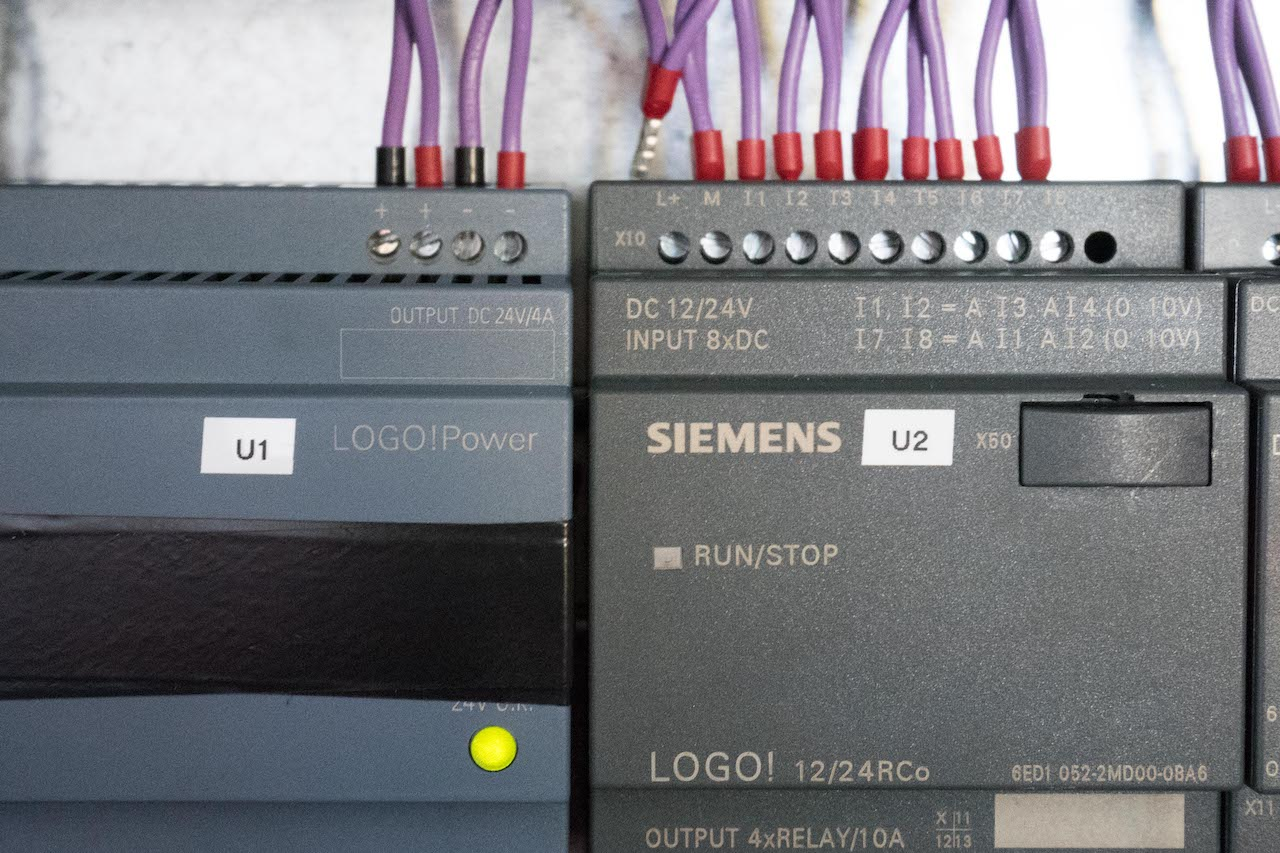
\includegraphics[width=0.7\linewidth]{figures/enclosure-controller-plc-disconnected.jpg}
%\end{center}
%\caption{The PLC U2 is deactivated by removing the two cables from the L+ terminal of U2.}
%\label{figure:enclosure-controller-plc-deactivated}
%\bigskip
%\begin{center}
%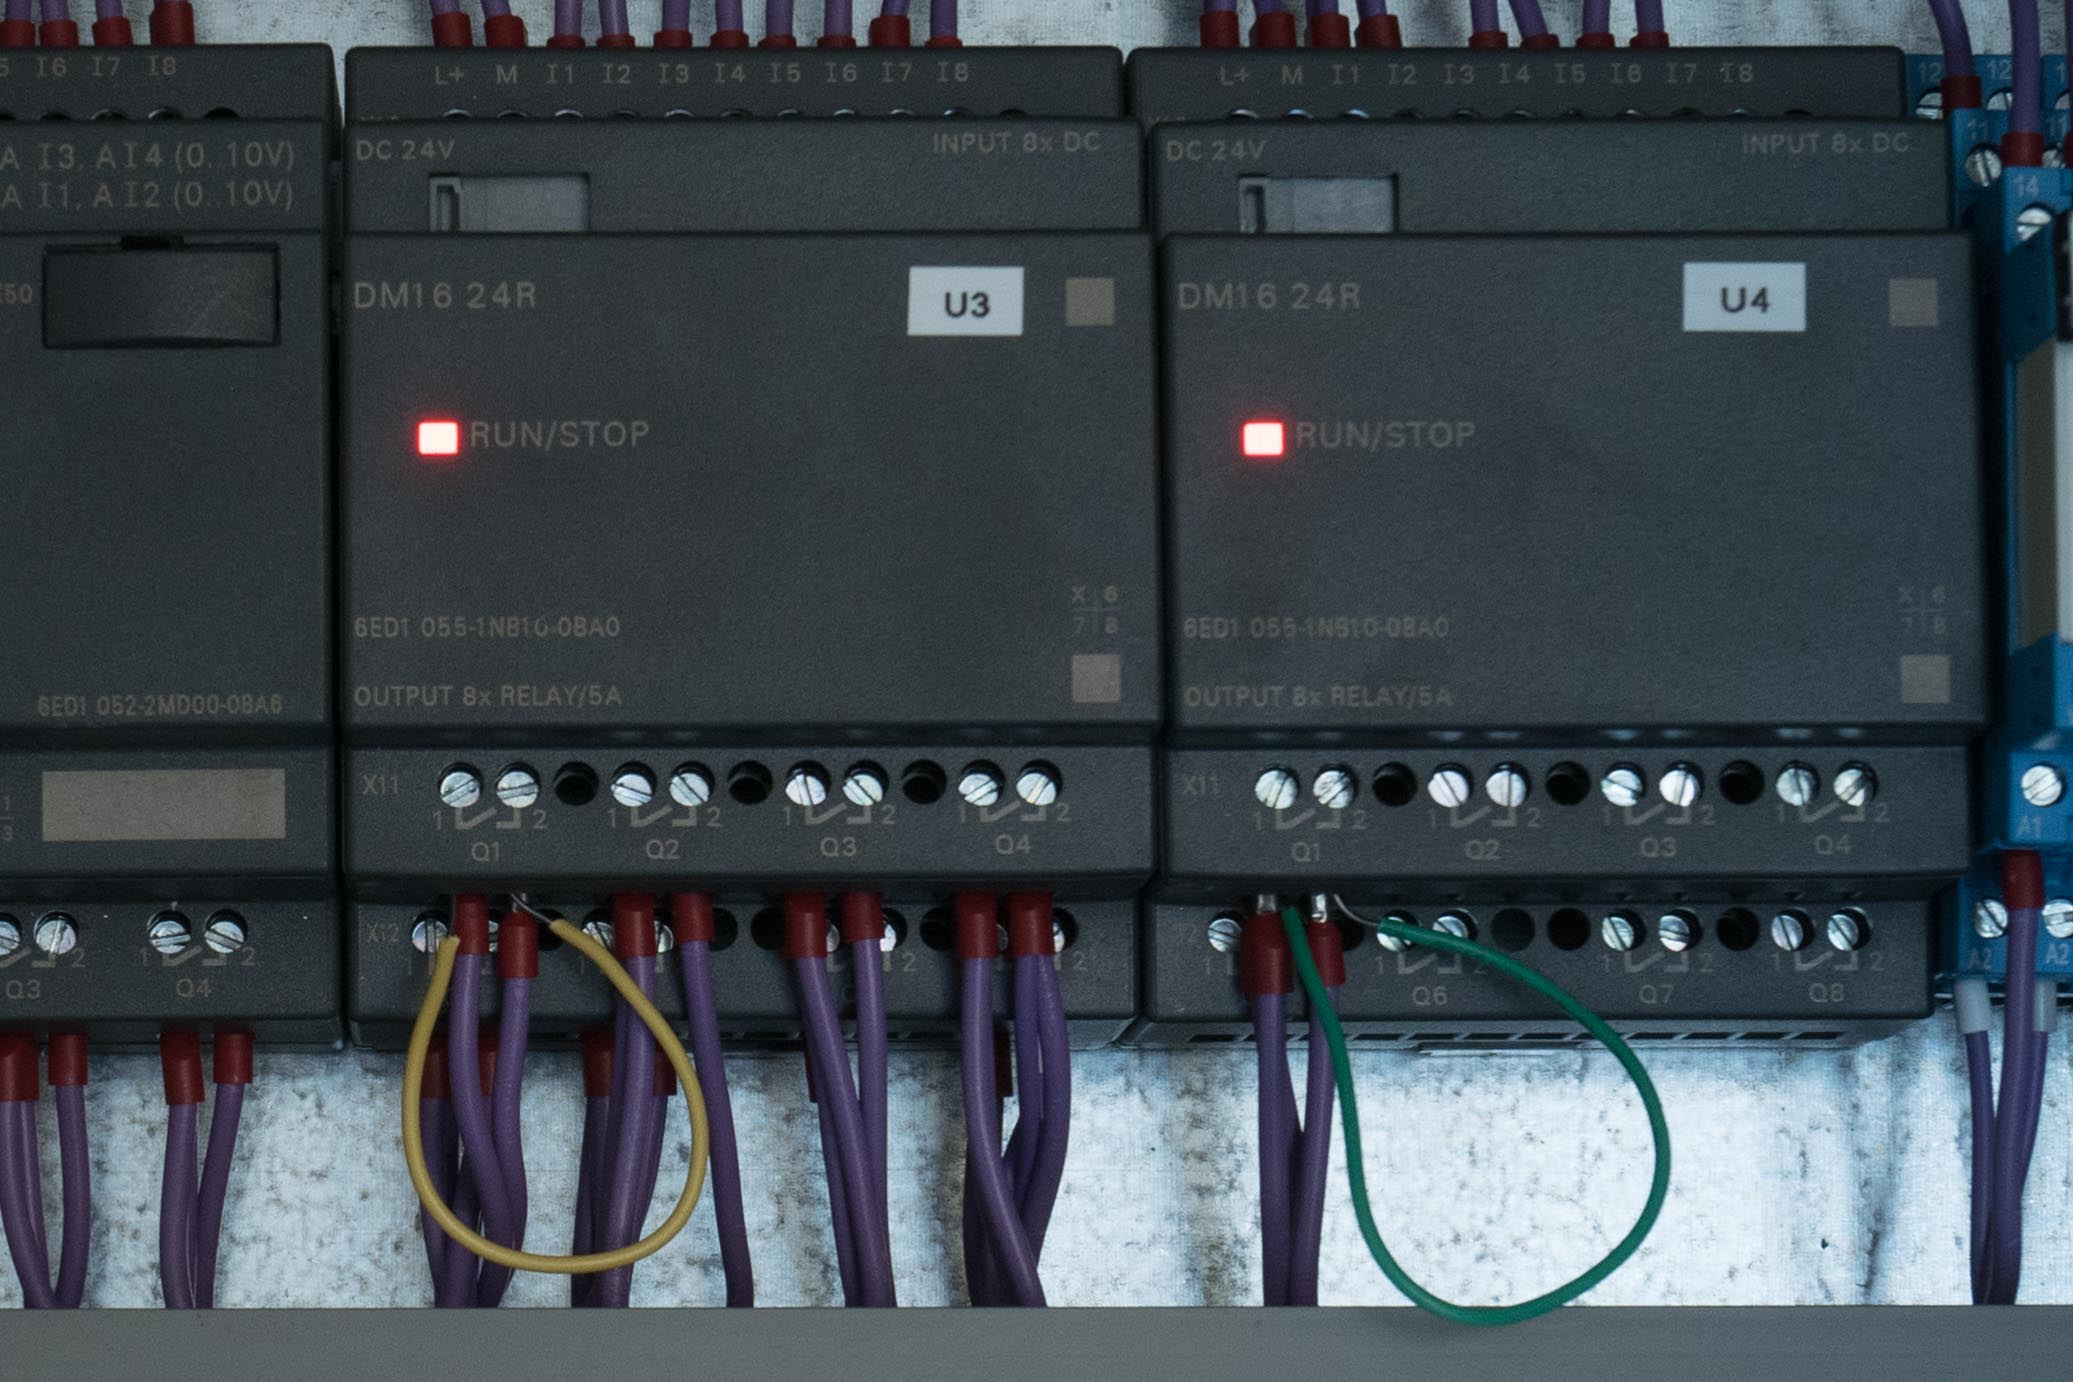
\includegraphics[width=0.7\linewidth]{figures/enclosure-controller-jumpers.jpg}
%\end{center}
%\caption{Jumpers shorting the PLC relays. The yellow jumper shorting Q1 of U3 deactivates the motor breaks. The green jumper shorting Q1 of U4 activates the electromagnetic lock.}
%\label{figure:enclosure-controller-jumpers}
%\end{figure*}
%
%\begin{figure*}
%\begin{center}
%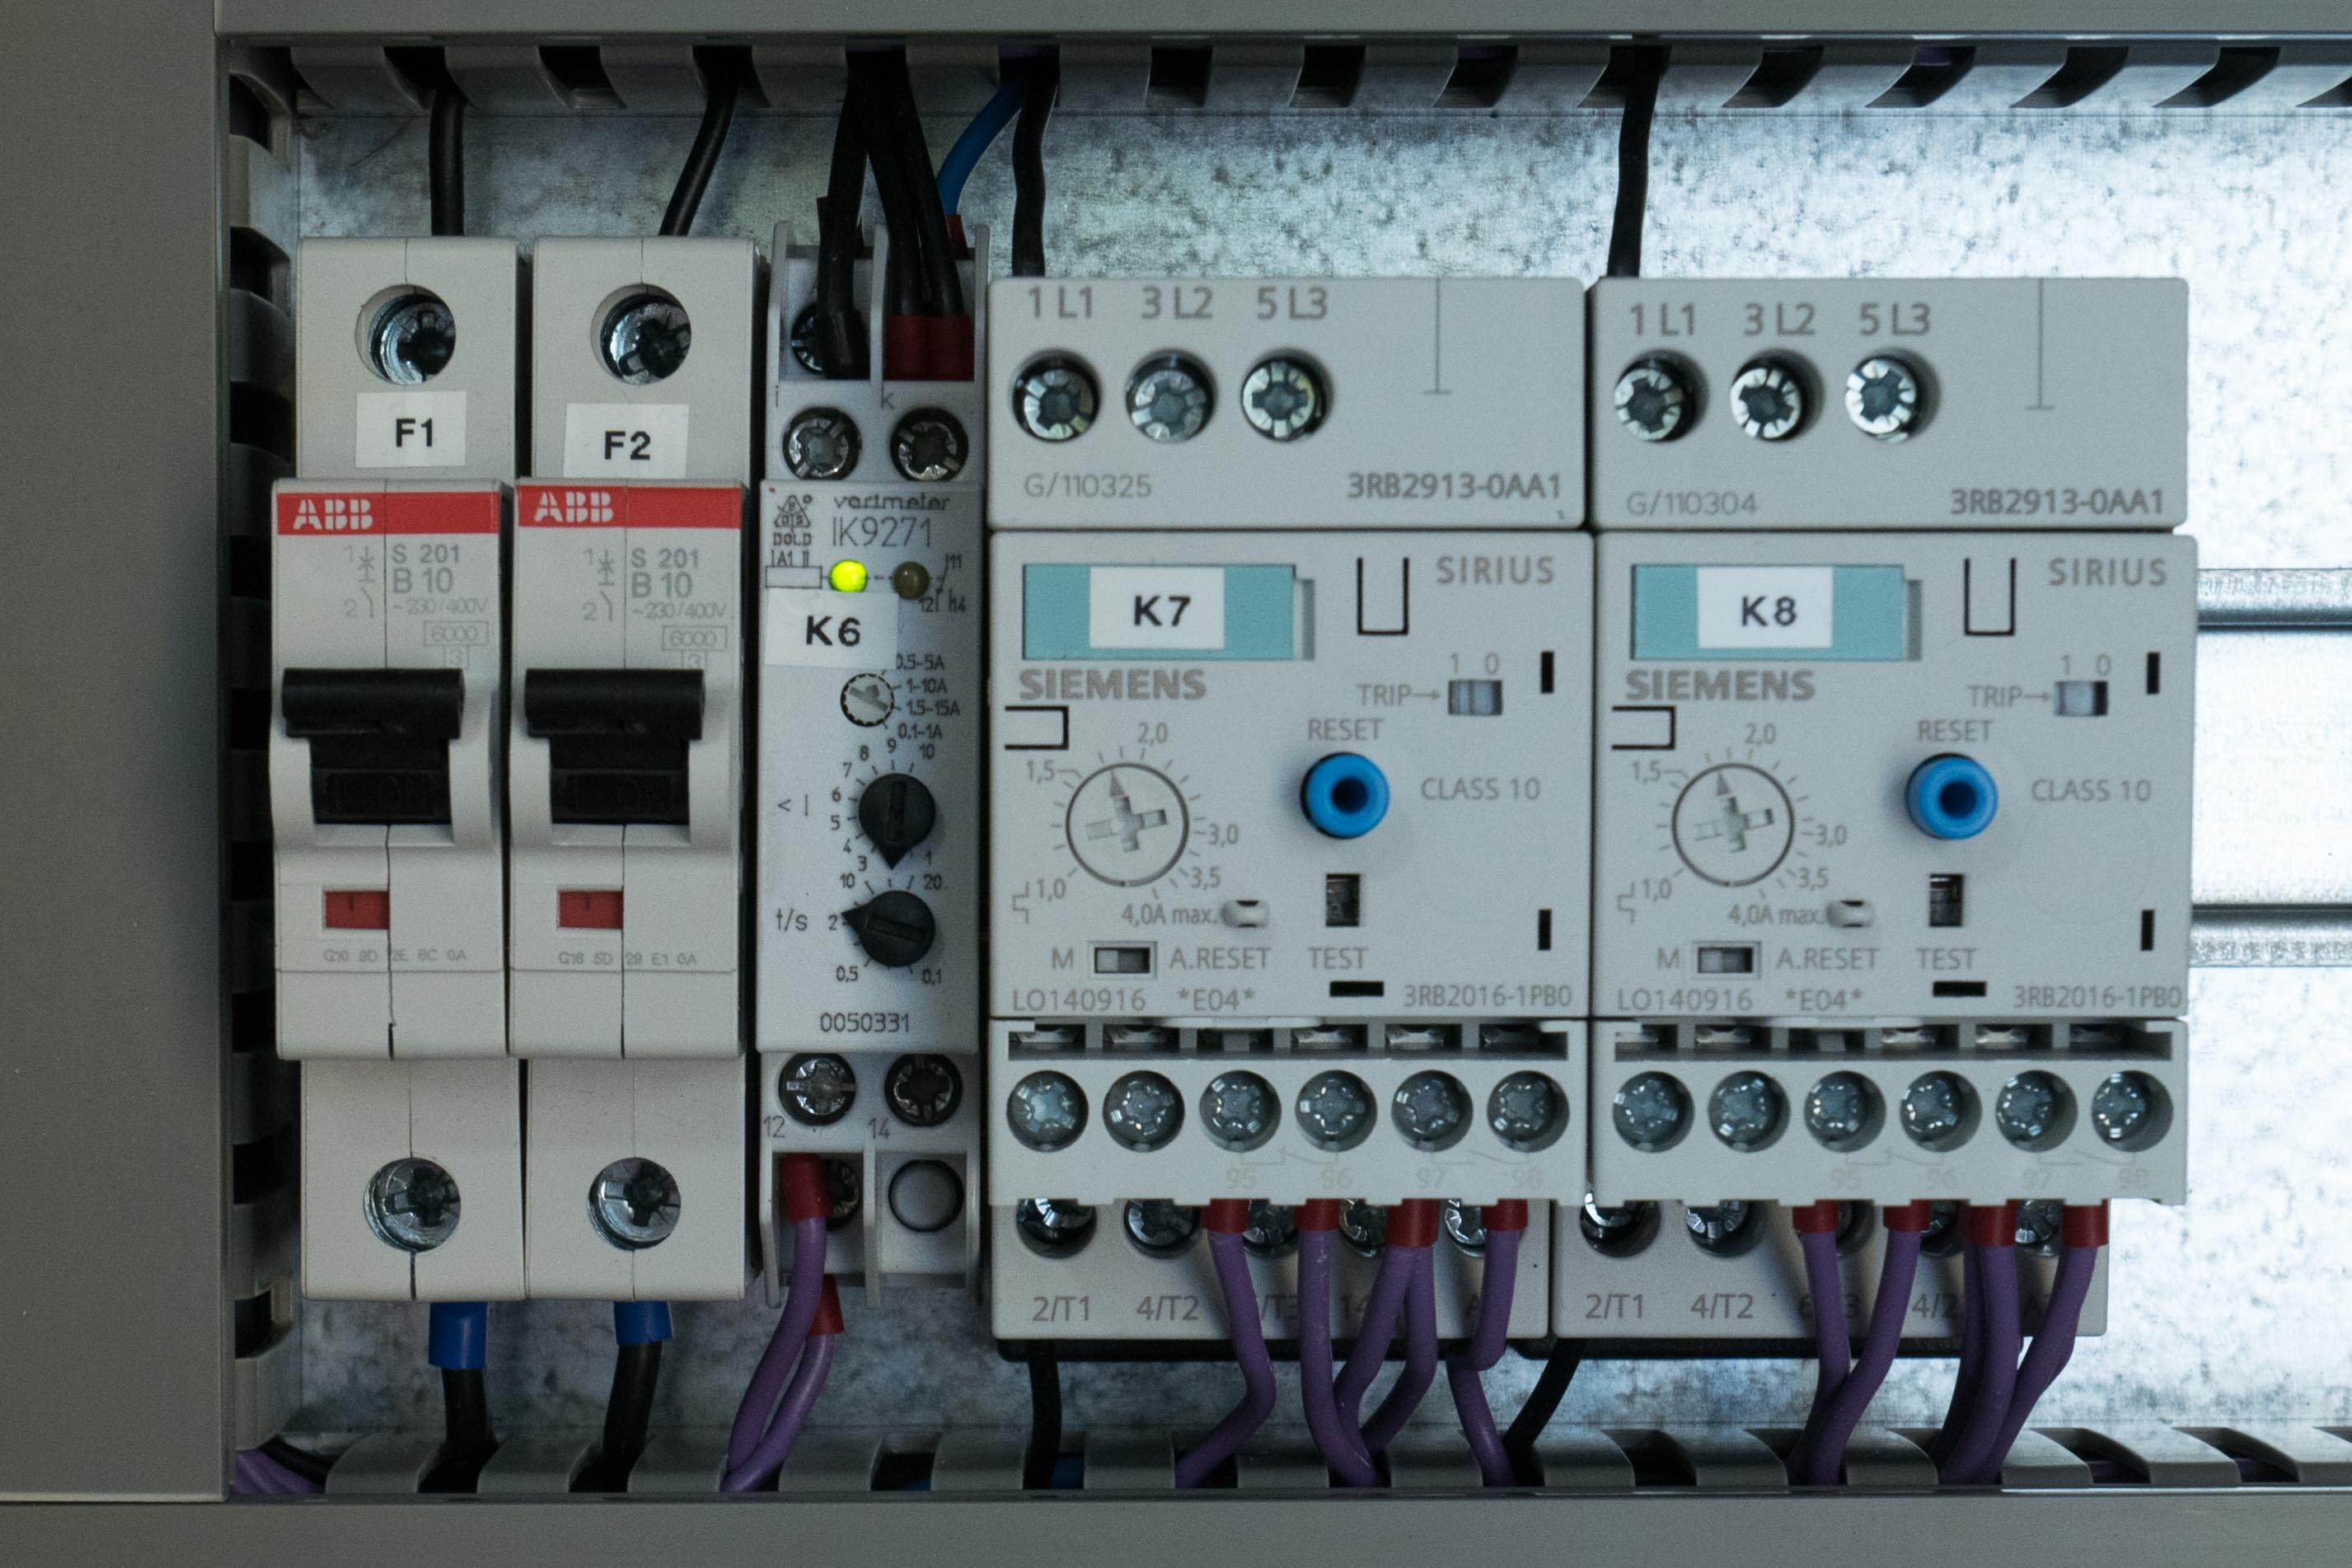
\includegraphics[width=0.7\linewidth]{figures/enclosure-controller-k6-activated.jpg}
%\end{center}
%\caption{The green LED on K6 lights up indicates that the motor brakes have been deactivated. The orange LED to the right of the green LED also lights up for a few seconds.}
%\label{figure:enclosure-controller-k6-activated}
%\bigskip
%\begin{center}
%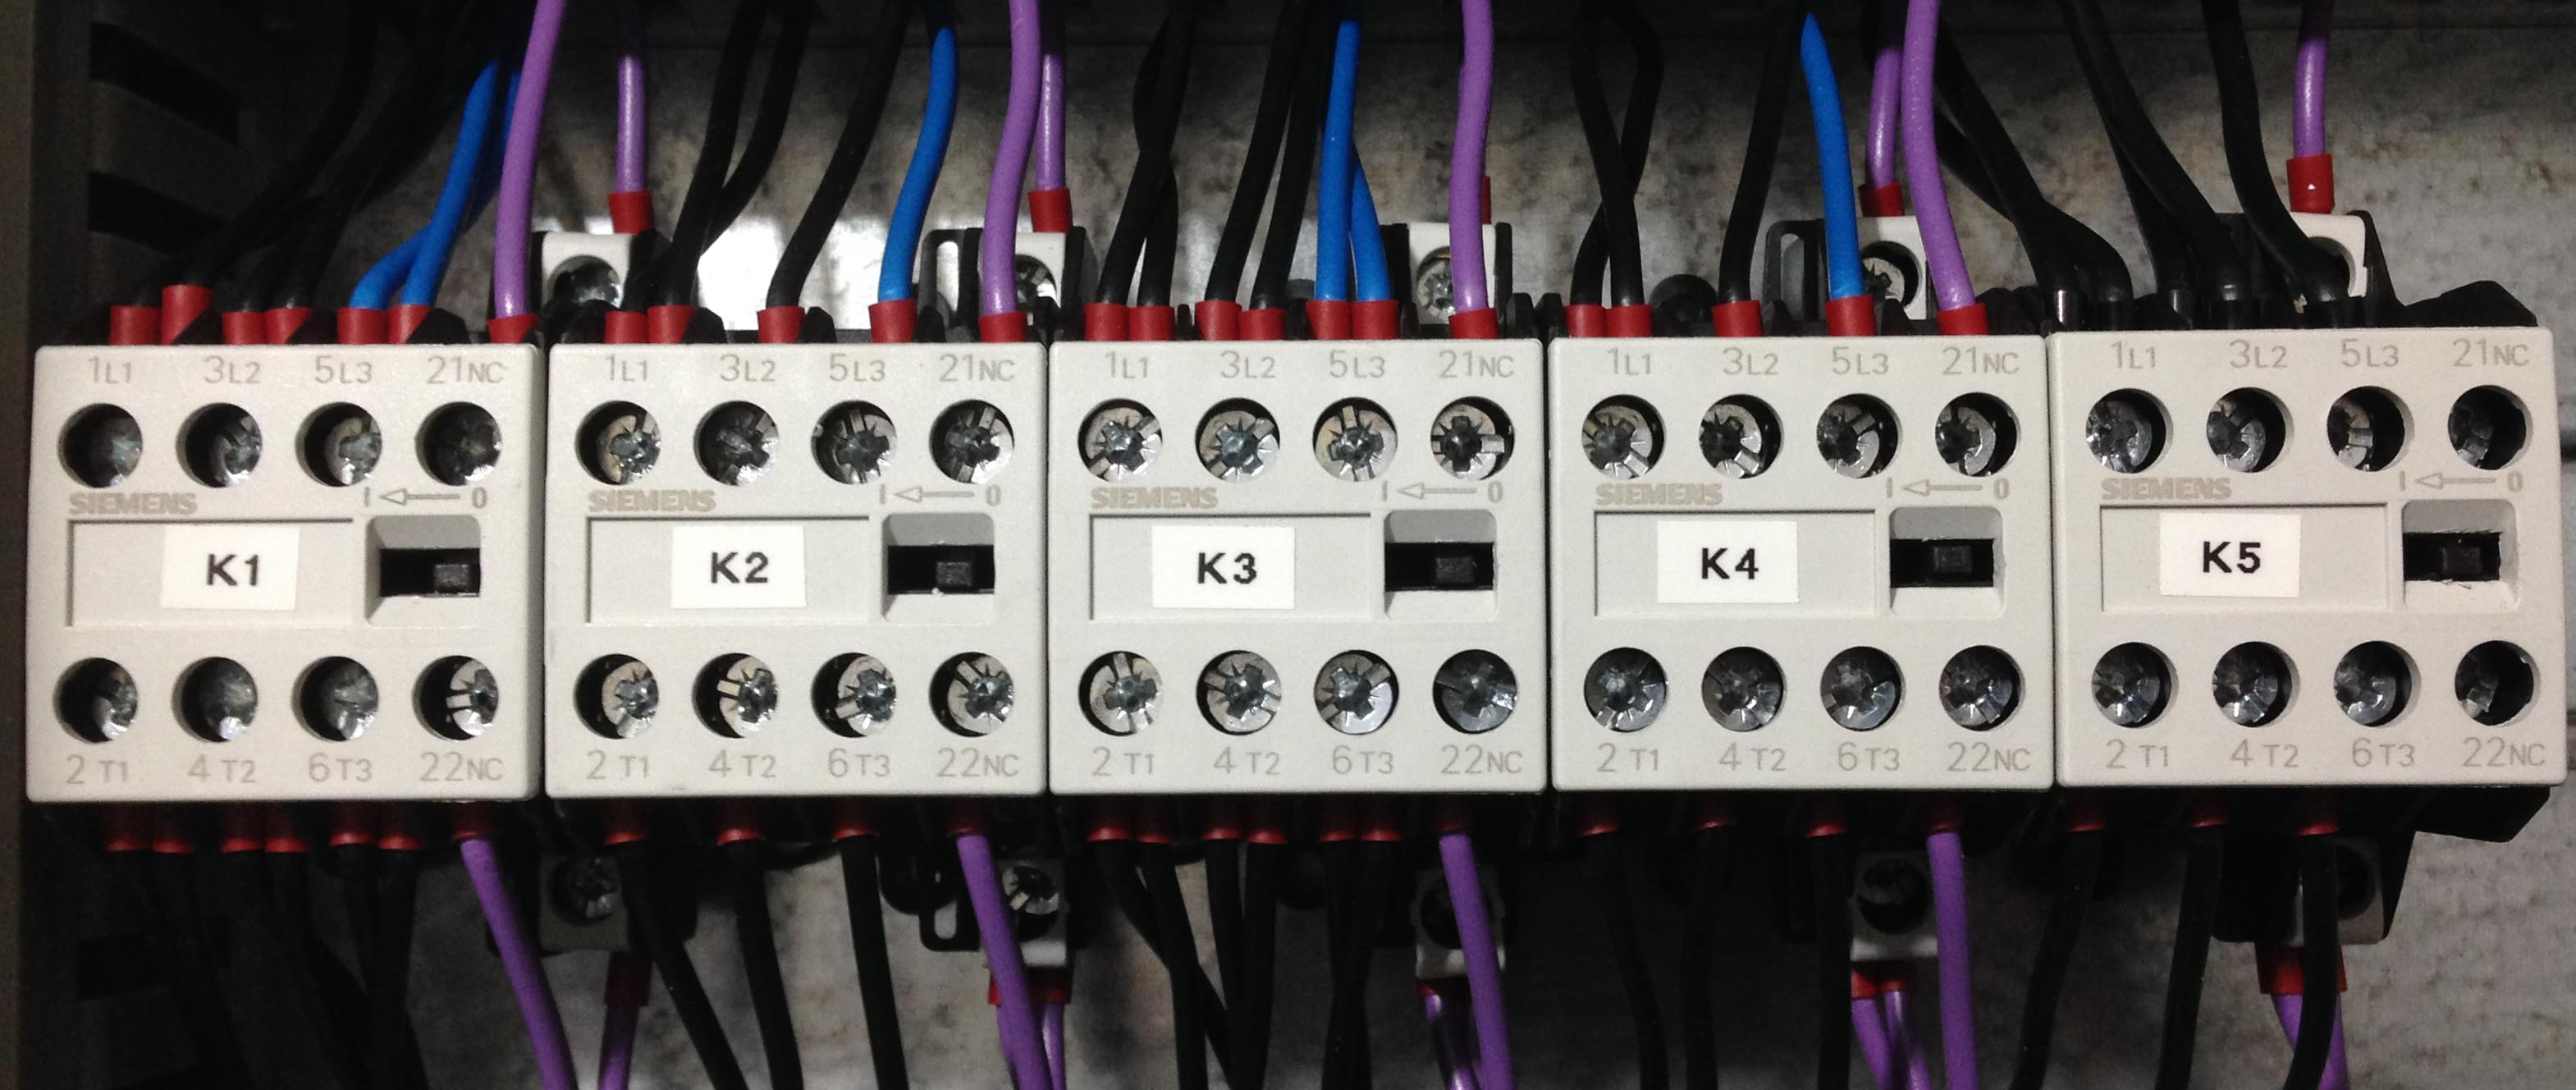
\includegraphics[width=0.8\linewidth]{figures/enclosure-controller-relays.jpg}
%\end{center}
%\caption{The relays that control the motors (K1 and K4 to close and K2 and K3 to open) and motor brakes (K5).}
%\label{figure:enclosure-controller-relays}
%\end{figure*}
%
%\begin{figure*}
%\begin{center}
%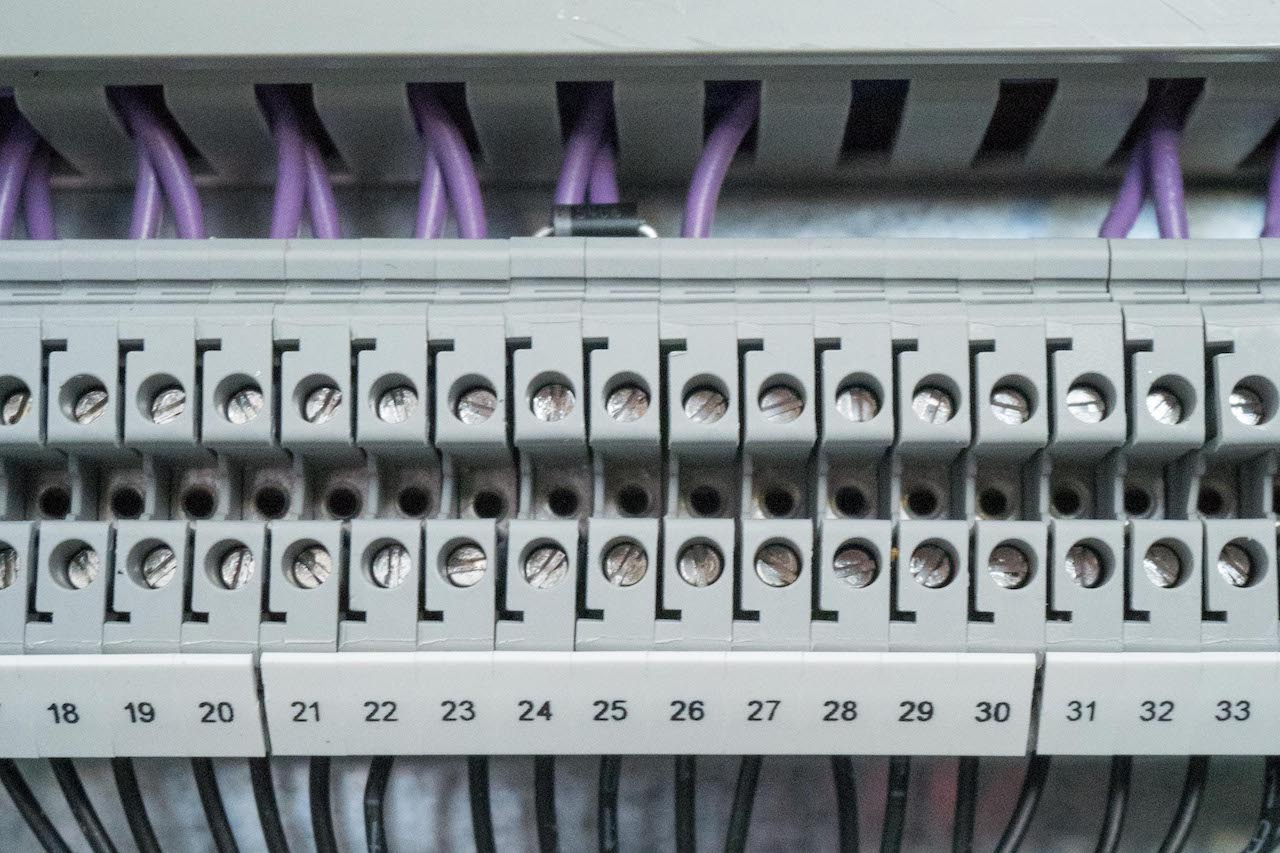
\includegraphics[width=0.7\linewidth]{figures/enclosure-controller-diode.jpg}
%\end{center}
%\caption{The diode across terminals 24 and 25 of the output connector. When the electromagnetic lock is activated, there are 24 VDC across the diode.}
%\label{figure:enclosure-controller-diode}
%\end{figure*}
%
%If power is available and the motors work, the enclosure can be opened and closed by manually activating the relays in the enclosure controller for the motor brakes, motors, and electromagnetic lock.
%
%This is not to be undertaken lightly, as there are risks both to personnel and equipment. First, these procedures require working in proximity to live 220 VAC. Second, many of the usual safety features that protect the equipment are not available. For example, if you accidentally activate the motor relays incorrectly, you can short the relays and will probably damage them.  For a similar reason, it is necessary to disable the PLC to avoid it attempting to activate the relays while they are being activated manually.
%
%\subsubsection{Safety Considerations}
%
%\safety{Be extremely careful when working inside the controller cabinet as it uses 220 VAC.}
%
%\subsubsection{Requirements}
%
%You will need:
%\begin{itemize}
%\item At least one person.
%\item Two small flat-headed screwdrivers.
%\item Two low-voltage jumper cables.
%\item A multimeter.
%\item The key to the shed (see \S\ref{section:shed-key}).
%\end{itemize}
%All of these can be found in the tool box in the {\projectname} equipment cabinet in the ground floor of the 84-cm telescope building.
%
%\subsubsection{Procedure for Closing the Enclosure}
%
%To close the enclosure:
%
%\begin{enumerate}
%\item
%Go to the shed.
%
%\item Switch off the enclosure controller.
%
%Move the main power switch on the controller door from ON to OFF.
%
%\item Deactivate the PLC.
%
%Remove the two cables from the L+ terminal of U2. See Figure~\ref{figure:enclosure-controller-plc-deactivated}.
%
%\item Prepare to deactivate the motor brakes.
%
%Short the Q1 relay of U3 using a jumper cable. See Figure~\ref{figure:enclosure-controller-jumpers}.
%
%\item Prepare to activate the electromagnetic lock.
%
%Short the Q1 relay of U4 using a jumper cable. See Figure~\ref{figure:enclosure-controller-jumpers}.
%
%\item Switch on the enclosure controller.
%
%Move the main power switch on the controller door from OFF to ON.
%
%\item 
%Check that the PLC is deactivated. 
%
%Check that the RUN/STOP LED on U2 does not light up. See Figure~\ref{figure:enclosure-controller-plc-deactivated}. (The RUN/STOP LEDs on U3 and U4 should light up.) If the LED on U2 does light up, you have not correctly disconnected its power. Start again.
%
%\item 
%Check that the motor breaks are deactivated. 
%
%Check that the green LED on K6 lights up to indicate that the motor brakes have been deactivated. The orange LED to the right of the green LED should also lights up for a few seconds. See Figure~\ref{figure:enclosure-controller-k6-activated}. If they do not do this, you have not correctly connected the jumper across the Q1 relay of U3. Start again.
%
%\item
%Check that the electromagnetic lock is activated. 
%
%Check that there is 24 VDC across the diode between terminal 24 and 25 of the output connector. See Figure~\ref{figure:enclosure-controller-diode}. If there is not, you have not correctly connected the jumper across the Q1 relay of U4. Start again.
%
%\item Run the motors to close the enclosure. 
%
%Use two screwdrivers to move the sliders of K1 and K4 from 0 to 1 and hold them there until the enclosure is closed. See Figure~\ref{figure:enclosure-controller-relays}. You may stop opening the enclosure at any point by releasing the sliders. Once the enclosure is fully closed you will hear the relays K9 and K10 activating and you should release the sliders. 
%
%\item Switch off the enclosure controller.
%
%Move the main power switch on the controller door from ON to OFF.
%
%\item Prepare to activate the motor brakes.
%
%Remove the jumper shorting Q1 of U3.
%
%\item Switch on the enclosure controller.
%
%Move the main power switch on the controller door from OFF to ON.
%
%\end{enumerate}
%
%\subsubsection{Procedure for Opening the Enclosure}
%
%To open the enclosure:
%
%\begin{enumerate}
%\item Switch off the enclosure controller.
%
%Move the main power switch on the controller door from ON to OFF.
%
%\item Deactivate the PLC.
%
%Remove the two cables from the L+ terminal of U2. See Figure~\ref{figure:enclosure-controller-plc-deactivated}.
%
%\item Prepare to deactivate the motor brakes.
%
%Short the Q1 relay of U3 using a jumper cable. See Figure~\ref{figure:enclosure-controller-jumpers}.
%
%\item Prepare to deactivate the electromagnetic lock.
%
%If you have previously activated the electromagnetic lock by shorting the Q1 relay of U4 using a jumper cable, remove the jumper cable. See Figure~\ref{figure:enclosure-controller-jumpers}.
%
%\item Switch on the enclosure controller.
%
%Move the main power switch on the controller door from OFF to ON.
%
%\item 
%Check that the PLC is deactivated. 
%
%Check that the RUN/STOP LED on U2 does not light up. See Figure~\ref{figure:enclosure-controller-plc-deactivated}. (The RUN/STOP LEDs on U3 and U4 should light up.) If the LED on U2 does light up, you have not correctly disconnected its power. Start again.
%
%\item 
%Check that the motor breaks are deactivated. 
%
%Check that the green LED on K6 lights up to indicate that the motor brakes have been deactivated. The orange LED to the right of the green LED should also lights up for a few seconds. See Figure~\ref{figure:enclosure-controller-k6-activated}. If they do not do this, you have not correctly connected the jumper across the Q1 relay of U3. Start again.
%
%\item
%Check that the electromagnetic lock is deactivated. 
%
%Check that there is 0 VDC across the diode between terminal 24 and 25 of the output connector. See Figure~\ref{figure:enclosure-controller-diode}. If there is not, you have not correctly disconnected the jumper across the Q1 relay of U4. Start again.
%
%\item Run the motors to open the enclosure. 
%
%Use two screwdrivers to move the sliders of K2 and K3 from 0 to 1 and hold them there until the enclosure is open. See Figure~\ref{figure:enclosure-controller-relays}. You may stop opening the enclosure at any point by releasing the sliders. Once the enclosure is fully open you will hear the relays K9 and K10 activating and you should release the sliders. 
%
%\item Switch off the enclosure controller.
%
%Move the main power switch on the controller door from ON to OFF.
%
%\item Prepare to activate the motor brakes.
%
%Remove the jumper shorting Q1 of U3.
%
%\item Switch on the enclosure controller.
%
%Move the main power switch on the controller door from OFF to ON.
%
%\end{enumerate}

\subsection{Manual Opening or Closing without Power}
\label{section:enclosure-manual-opening-or-closing-without-power}

If the enclosure cannot be operated normally using remote mode or local mode, you can bypass the control system and operate it manually by driving the motor axles manually with portable electric drills. This procedure requires two people. 

%There are two modes, depending on whether power is available. Here we document the procedure for opening or closing without power. In \S\ref{section:enclosure-manual-opening-or-closing-with-power} we documented the procedure for opening or closing with power.

This is not to be undertaken lightly, as it involves working on the balcony. However, when carried out with appropriate safety precautions and with calm, it is quite safe.

\subsubsection{Safety Considerations}

\safety{Be extremely careful when working inside the controller cabinet as it uses 220 VAC.}

\safety{Use a harness, line, and helmet when you work on the platform or balconies.}

\subsubsection{Requirements}

You will need:

\begin{itemize}
\item Two people.
\item Two portable electrical drills with 6 mm hex drives.
\item The key to the shed (see \S\ref{section:shed-key}).
\end{itemize}

Two suitable drills with drives are stored in the {\projectname} equipment cabinet in the ground floor of the 84-cm telescope building. The batteries are normally connected to wall socket.

\subsubsection{Procedure for Closing the Enclosure}


\begin{figure*}
\begin{center}
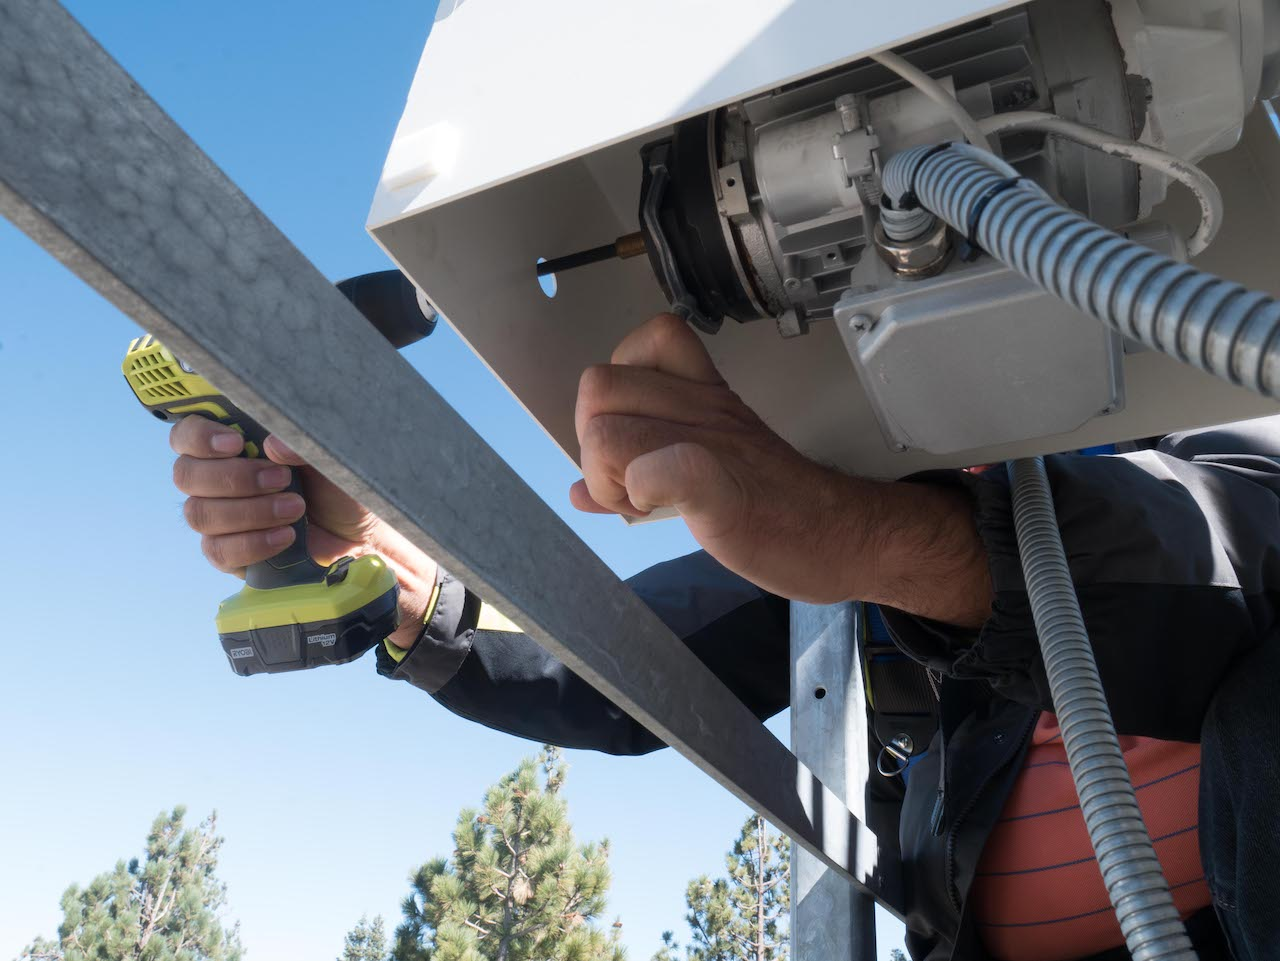
\includegraphics[width=0.7\linewidth]{figures/enclosure-closing-with-drills.jpg}
\end{center}
\caption{Opening or closing the enclosure with portable electric drills. The motor brake is disengaged by pushing the lever under the motor away from the platform.}
\label{figure:enclosure-closing-with-drills}
\end{figure*}

To close the enclosure:

\begin{enumerate}
\item Switch off the enclosure controller.

Move the main power switch on the controller door from ON to OFF.

%\item Deactivate the PLC.
%
%Remove the two cables from the L+ terminal of U2. See %Figure~\ref{figure:enclosure-controller-plc-deactivated}.

%\item Prepare to activate the electromagnetic lock.
%
%Short the Q1 relay of U4 using a jumper cable. See Figure~\ref{figure:enclosure-controller-jumpers}.

%\item Switch on the enclosure controller.
%
%Move the main power switch on the controller door from OFF to ON.

%\item 
%Check that the PLC is deactivated. 
%
%Check that the RUN/STOP LED on U2 does not light up. See Figure~\ref{figure:enclosure-controller-plc-deactivated}. (The RUN/STOP LEDs on U3 and U4 should light up.) If the LED on U2 does light up, you have not correctly disconnected its power. Start again.

%\item
%Check that the electromagnetic lock is activated. 
%
%Check that there is 24 VDC across the diode between terminal 24 and 25 of the output connector. See Figure~\ref{figure:enclosure-controller-diode}. If there is not, you have not correctly connected the jumper aross the Q1 relay of U4. Start again.


\item
Use appropriate safety equipment: harnesses, lines, and helmets. These are found in the shed.

\item
One person should ascend to one balcony with one drill and the other person to the other balcony with the other drill.

\item
Use your safety line to secure yourself to the balcony rail. Loop the line over the rail and then fasten the clasp on the line itself.

\item
Set the direction of the drill appropriately to close the enclosure.

\item
Insert the drill into the motor axle. See Figure~\ref{figure:enclosure-closing-with-drills}.

\item
Push the lever underneath the motor away from the platform to release the brake. Keep the brake released and run the electric drill to turn the motor axle. The two people should do this relatively slowly and coordinate; if one gets too far ahead of or behind the other, you can damage the arch or bearing.

\item
Once the enclosure is closed, release the brake lever, remove the drills, and descend from the platform.

\item
Open the enclosure controller.

\item
Engage the manual lock. This switches on the enclosure electromagnet and actuates the enclosure emergency stop buttons. This ensures that the electromagnet stays energized even if the PLC fails and that the PLC cannot attempt to open the enclosure.

Move the manual lock switch inside the enclosure controller from OFF to ON. See Figure~\ref{figure:enclosure-controller-manual-lock-switch}.

\item
Close the enclosure controller.

\item
Switch on the enclosure controller.

Move the main power switch on the controller door from OFF to ON.

\item
Place the enclosure in remote mode.

Move the enclosure controller mode selector switch to “REMOTE”.

\end{enumerate}

\subsubsection{Procedure for Opening the Enclosure}

To open the enclosure:

\begin{enumerate}
\item Switch off the enclosure controller.

Move the main power switch on the controller door from ON to OFF.

\item
Open the enclosure controller.

\item
Disengage the manual lock.

Move the manual lock switch inside the enclosure controller from ON to OFF. See Figure~\ref{figure:enclosure-controller-manual-lock-switch}.

\item
Close the enclosure controller.

\item
Use appropriate safety equipment: harnesses, lines, and helmets. These are found in the shed.

\item
One person should ascend to the northern balcony with one drill and one to the southern balcony with the other drill.

\item
Use your safety line to secure yourself to the balcony rail. Loop the line over the rail and then fasten the clasp on the line itself.

\item
Set the direction of the drill appropriately to open the enclosure.

\item
Insert the drill into the motor axle. See Figure~\ref{figure:enclosure-closing-with-drills}.

\item
Push the lever underneath the motor away from the platform to release the brake. Keep the brake released and run the electric drill to turn the motor axle. The two people should do this relatively slowly and coordinate; if one gets too far ahead of or behind the other, you can damage the arch or bearing.

\item
Once the enclosure is open, release the brake lever, remove the drills, and descend from the platform.

\item
Switch on the enclosure controller.

Move the main power switch on the controller door from OFF to ON.

\end{enumerate}

\subsection{Shutting-Down Before and Starting-Up After the Winter Break}
\label{section:enclosure-manual-winter-break}

The observatory and {\projectname} cease operations during a winter break of about three weeks. During the winter break the enclosure should be left closed and powered on but with a hardware override on the electromagnetic lock.

\subsubsection{Safety Considerations}

\safety{Be extremely careful when working inside the controller cabinet as it uses 220 VAC.}

\subsubsection{Requirements}

You will need:
\begin{itemize}
\item At least one person.
\item The key to the shed (see \S\ref{section:shed-key}).
\end{itemize}
All of these can be found in the tool box in the {\projectname} equipment cabinet in the ground floor of the 84-cm telescope building.

\subsubsection{Procedure for Shutting-Down Before the Winter Break}

To prepare the enclosure before the winter break:

\begin{enumerate}
\item
Go to the shed.

\item
Move the enclosure controller mode selector switch to “LOCAL”.

\item If the weather permits, open the enclosure to 60 $\deg$.

Set the angle selector switch to the 60 $\deg$ and then press and hold the open button until the green light goes out.

\item Close the dome.

Press and hold the close button until the green light goes out.

\item Switch off the enclosure controller.

Move the main power switch on the controller door from ON to OFF.

\item
Open the enclosure controller.

\item
Engage the manual lock. This switches on the enclosure electromagnet and actuates the enclosure emergency stop buttons. This ensures that the electromagnet stays energized even if the PLC fails and that the PLC cannot attempt to open the enclosure.

Move the manual lock switch inside the enclosure controller from OFF to ON. See Figure~\ref{figure:enclosure-controller-manual-lock-switch}.

\item
Close the enclosure controller.

\item Leave the enclosure controller mode selector switch to “LOCAL”.

\end{enumerate}

\subsubsection{Procedure for Starting-Up After the Winter Break}

To prepare the enclosure after the winter break:

\begin{enumerate}
\item
Go to the shed.

\item Switch off the enclosure controller.

Move the main power switch on the controller door from ON to OFF.

\item Open the enclosure controller.

\item
Disengage the manual lock.

Move the manual lock switch inside the enclosure controller from ON to OFF. See Figure~\ref{figure:enclosure-controller-manual-lock-switch}.

\item
Close the enclosure controller.

\item Switch on the enclosure controller.

Move the main power switch on the controller door from OFF to ON.

\item Move the enclosure controller mode selector switch to “REMOTE”.

\end{enumerate}

\section{Remote Interface}

\subsection{Lantronix EDS}

The RS-232 interface to the enclosure controller is made available via the Lantronix EDS 4100 ethernet-to-serial converter. Specifically, it is connected to line 3 and configured as 9600/8-N-1 with a tunnel on TCP port 10003.

The Lantronix EDS is on the LAN at \verb|serial|.

\subsection{ADAM Modules}
\label{section:enclosure-adam-modules}

Remote control of the enclosure is through an ADAM-4055 digital input/output module. The input and output channels of the ADAM-4055 module are connected to the enclosure controller PLC.

The RS-485 serial interface of the ADAM-4055 is exposed via an ADAM-4520 RS-232 to RS-485 converter and isolator as RS-232 at 9600/8-N-1.

The state of the input and output channels can be determined either from the web interface (the “Input Channels” and “Output Channels” variables in the “Enclosure” tab) or by unscrewing the ADAM-4520 RS-232 to RS-485 converter on top of the ADAM-4055 to reveal LEDs which show the state of the channels.

The input channels are:
\begin{description}
\item[DI0] Open. 0 = not open and 1 = open. This channel is connected to terminal U3/Q5 (“Kuppel AUF”) on the PLC. Its value is determined by the PLC from the proximity switches on the platform.
\item[DI1] Closed. 0 = not closed and 1 = closed. This channel is connected to terminal U3/Q6 (“Kuppel ZU”) on the PLC. Its value is determined by the PLC from the proximity switches on the platform.
\item[DI2] Error. In remote mode, 1 = error and 0 = no error. In local mode, this follows the state of the red error button (constant 0 = not error, constant 1 = emergency stop button pressed, and intermittent at 1, 2, or 4 Hz for under-current, over-current, and safety rail errors). This channel is connected to U3/Q4 (“Störung”) on the PLC, which also control the red error button. Its value is determined by the PLC. Note that the behavior of this channel in local mode makes it only useful in remote mode.
\item[DI3] Mode. 0 = local and 1 = remote. This channel is connected to terminal U4/I2 (“Hand/Auto”) of the PLC. Its value is directly determined by the mode switch. 
\item[DI4] Motor over-current error. 0 = no error and 1 = error. This channel is connected to terminal U3/I7 (“Motorschutz”) of the PLC. Its value is directly determined by the motor over-current relays K7 and K8.
\item[DI5] Rain sensor. 0 = dry and 1 = wet. This channel is connected to terminal U3/Q8 (“Regensensor”) on the PLC. Its value is determined by the PLC from the rain sensor switch on the platform. 
\item[DI6] Safety strip. 0 = not pressed and 1 = pressed. This channel is connected to terminal U4/I1 (“Dichtlippe”) on the PLC. Its value is directly determined by the safety rail switch.
\item[DI7] Emergency stop. 0 = not pressed and 1 = pressed. This channel is not connected to the PLC but rather to the emergency stop button circuit. Its value is determined directly by the emergency stop buttons.
\end{description}

The output channels are:
\begin{description}
\item[DO0] Open. In remote mode, set to 1 to open to the position specified by DO3, DO4, and DO5. This channel is connected to terminal U2/I3 (“AUF”) of the PLC via relay K11.
\item[DO1] Close. In remote mode, set to 1 to close. This channel is connected to terminal U2/I4 (“ZU”) of the PLC via relay K12.
\item[DO2] Reset. In remote mode, set to 1 to reset an error. This channel is connected to terminal U2/I8 (“Reset”) of the PLC via relay K13.
\item[DO3] 60 deg. Set to 1 to select 60 degrees. This channel is connected to terminal U4/I5 (“Auto 60-Grad”) of the PLC via relay K14.
\item[DO4] 90 deg. Set to 1 to select 90 degrees. This channel is connected to terminal U4/I6 (“Auto 90-Grad”) of the PLC via relay K15. 
\ifcoatli
(The {\projectname} enclosure does not have hardware to open to 90 degrees.)
\fi
\item[DO5] 120 deg. Set to 1 to select 120 degrees. This channel is connected to terminal U4/I7 (“Auto 120-Grad”) of the PLC via relay K16.
\item[DO6] Not used.
\item[DO7] Not used.
\end{description}

If D03, D04, and D05 are all set to 0, opening will open to 180 degrees. 
\ifcoatli
The {\projectname} enclosure has hardware to support opening to 60, 120, and 180 degrees; it does not have hardware to support opening to 90 degrees. 
\fi
\ifddoti
The {\projectname} enclosure has hardware to support opening to 60, 90, 120, and 180 degrees.
\fi

\subsection{Diagnostics}

To check communication with the Lantronix EDS, from a terminal run:

\begin{quotation}
\begin{verbatim}
ping serial
\end{verbatim}
\end{quotation}

To check communication with the ADAM modules, from a terminal on \verb|control|, first stop the enclosure server so that it releases the enclosure TCP port on the Lantronix EDS:

\begin{quotation}
\begin{verbatim}
sudo stopserver enclosure
\end{verbatim}
\end{quotation}

Then connect to the enclosure TCP port on the Lantronix EDS using telnet:

\begin{quotation}
\begin{verbatim}
telnet serial 10003
\end{verbatim}
\end{quotation}

You can then send commands to the ADAM-4055. Some useful commands (which should be followed by ENTER) are:

\begin{itemize}
\item Command: \verb|$01M|

Response: \verb|!014055|

Read Module Name. The response shown above confirms that you are talking to an ADAM-4055.

\item 
Command: \verb|$016|

Response: \verb|!|$XXYY$\verb|00|

Digital Data In. The values of the output channels (in upper-case hexadecimal) are given by $XX$ and the values of the input channels (in upper-case hexadecimal) are given by $YY$.

\item 
Command: \verb|#0100|$XX$

Response: \verb|>|

Digital Data Out. The output channels are set to $XX$ (in upper-case hexadecimal).

\end{itemize}

For more details of the commands, see the ADAM-4000 Manual.

You can exit from telnet by typing CTRL-\verb|]| and then \verb|quit|. Once you have done so, you should probably restart the enclosure server on \verb|control| with:

\begin{quotation}
\begin{verbatim}
sudo startserver enclosure
\end{verbatim}
\end{quotation}

\begin{figure*}
\begin{center}
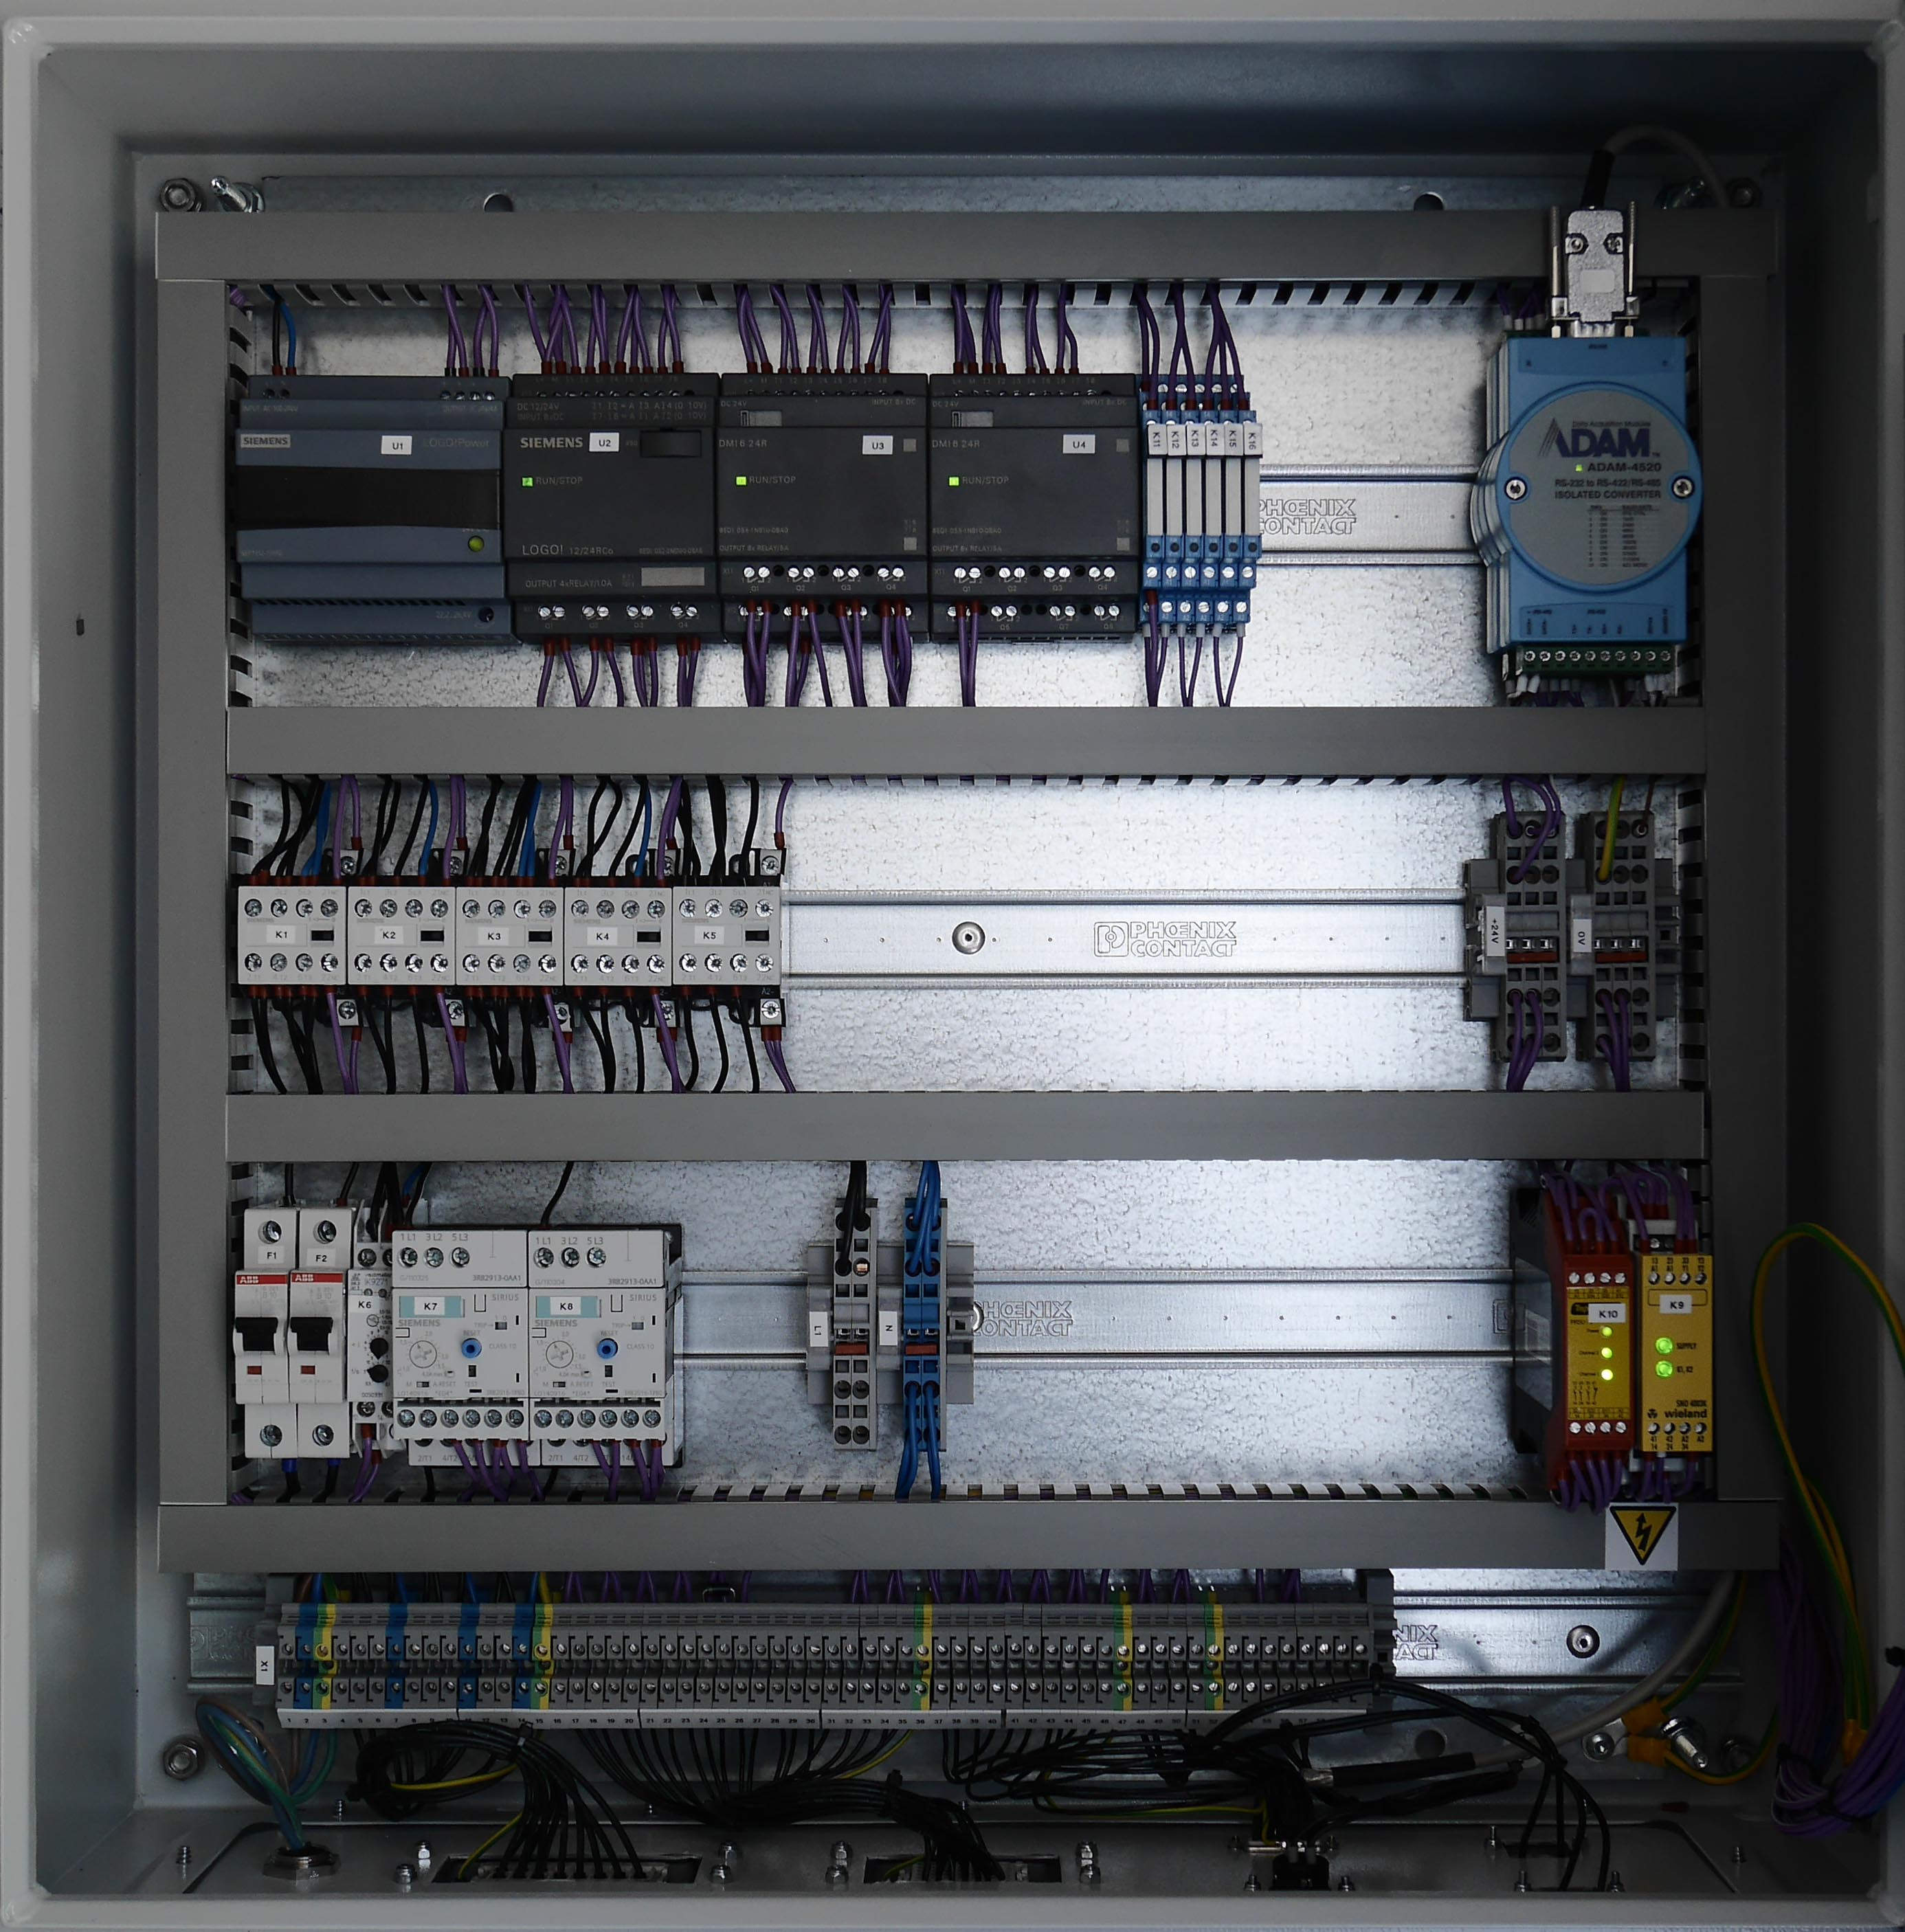
\includegraphics[width=\linewidth]{figures/enclosure-controller-inside.jpg}
\end{center}
\caption{The Enclosure Controller. Top rail, left to right: U1 is the power supply for the PLC; U2 is the PLC; U3 and U4 are extension units for the PLC; K11 to K16 are relays to convert between ADAM and PLC signal levels; finally two stacked ADAM modules. Middle rail, left to right: K1 to K4 are relays for the motors; K5 is the relay for the motor brakes; and +24 VDC and 0 VDC distribution blocks. Bottom rail, left to right: F1 and F2 are breakers for the motors; K6 is the delay relay to run the motors for a few seconds one the enclosure is open in order to synchronize the motors; K7 and K8 are motor over-current relays; 220 VAC live and neutral distribution blocks; K10 is XXX; and K9 is XXX.}
\label{figure:enclosure-controller-inside}
\end{figure*}

\begin{table*}
\caption{Enclosure Controller Components}
\begin{center}
\begin{tabular}{ll}
\hline
Code&Component\\
\hline
K6&Dold IK9217\\
K7/K8&Siemens 3RB2016-1PB0\\
     &Siemens 3RB2913-0AA1\\
\hline
\end{tabular}
\end{center}
\end{table*}

\section{Control}

The server for the enclosure runs on \verb|control|. 

The server starts automatically after \verb|control| is boots, but if necessary can be stopped, started, or restarted explicitly by issuing the following shell commands on \verb|control|:
\begin{itemize}
\item
\verb|sudo stopserver enclosure|
\item
\verb|sudo startserver enclosure|
\item
\verb|sudo restartserver enclosure|
\end{itemize}

Server requests can be issued from any of the Mac or Linux machines on the LAN. The following requests are supported:

\begin{itemize}
\item
\verb|request enclosure initialize|

Initialize the server and enclosure hardware. As part of the process of initializing, the enclosure will close.

For this request to be accepted, the server activity must not be \verb|starting| or \verb|error|.

If the request is accepted, the server activity changes to \verb|initializing| and then, once it has initialized, to \verb|idle|.

\item
\verb|request enclosure open| \var{angle}

Open the enclosure to the specified \var{angle}. If \var{angle} is omitted, a default value of \verb|180| is assumed.

Valid values of \var{angle} are \verb|60|, \verb|120|, and \verb|180|.

For this request to be accepted, the server activity must not be \verb|starting|, \verb|started|, \verb|initializing|, or \verb|error|.

If the request is accepted, the server activity changes to \verb|opening| and then, once it has opened to the specified angle, to \verb|idle|.

\item
\verb|request enclosure close|

Close the enclosure.

For this request to be accepted, the server activity must not be \verb|starting|, \verb|started|, \verb|initializing|, or \verb|error|.

If the request is accepted, the server activity changes to \verb|closing| and then, once it has closed, to \verb|idle|.

\item
\verb|request enclosure stop|

Stop the enclosure.

For this request to be accepted, the server activity must not be \verb|starting| or \verb|error|.

If the request is accepted, the server activity changes to \verb|stopping| and then, once it has stopped, to \verb|started| (if the server has not been initialized) or to the activity after the previous completed request.

\item
\verb|request enclosure reset|

Reset an error in the enclosure.


\item
\verb|request enclosure status|

Show the status of the server.

Obtain the values of the status data from the server and print them to stdout.
\end{itemize}

\section{Bibliography}

\begin{flushleft}
\begin{itemize}
\item “\href{bibliography/astelco-enclosure-data-sheet.pdf}{Technical Specifications: ASTELCO Remote Telescope Station (ARTS)}”, ASTELCO, Version V-1304-21.
\item “\href{bibliography/astelco-enclosure-technical-reference-manual.pdf}{Foldable Enclosure ENCL-ALTS-01 Technical Reference Manual}”, ASTELCO, Revision V-1.4.
\begin{itemize}
\item The statement that the enclosure used 230 V 50 Hz is not applicable. The {\projectname} and DDOTI/OAN enclosures use 220 V 60 Hz phase-phase.
\item The description of the ADAM input and output channels on page 19 is not applicable. The correct description is given in \S\ref{section:enclosure-adam-modules}.
\item 
\ifcoatli
The {\projectname} enclosure has hardware to support opening to 60, 120, and 180 degrees; it does not have hardware to support opening to 90 degrees. 
\fi
\ifddoti
The {\projectname} enclosure has hardware to support opening to 60, 90, 120, and 180 degrees.
\fi
\end{itemize}
\item \href{bibliography/astelco-enclosure-electronics-schematics.pdf}{Electronic Schematics}, ASTELCO, Revision A (in German).
\item \href{bibliography/astelco-enclosure-drawing-0500.pdf}{Drawing 0500 -- Enclosure Platform}, ASTELCO.
\item \href{bibliography/astelco-enclosure-drawing-5772.pdf}{Drawing 5772 -- Enclosure Tower Base Plates}, ASTELCO.
\item \href{bibliography/astelco-enclosure-drawing-5798.pdf}{Drawing 5798 -- Enclosure Tower}, ASTELCO.
\item \href{bibliography/astelco-enclosure-drawing-6610.pdf}{Drawing 6610 -- Enclosure Tower on Columns}, ASTELCO.
\item \href{bibliography/astelco-enclosure-drawing-6658.pdf}{Drawing 6658 -- Enclosure Tower on Columns}, ASTELCO.
\item \href{bibliography/astelco-enclosure-drawing-6662.pdf}{Drawing 6662 -- Interface with Columns}, ASTELCO.
\item “\href{bibliography/lantronix-eds-user-guide.pdf}{Lantronix EDS Device Servers/Terminal Servers User Guide}”, Lantronix, Revision 1 April 2011.
\item “\href{bibliography/advantech-adam-4000.pdf}{ADAM-4000 Data Adquisition Modules User's Guide]}”, Advantech, Edition 10.5, 2007.
\end{itemize}
\end{flushleft}